\chapter{Search Trees}

%%% Local Variables:
%%% mode: latex
%%% TeX-master: "book"
%%% End:

%\setcounter{chapter}{1}
%\newcommand{\hatcolon}{\hatChar \hskip-0.4em :}
%\newcommand{\hatminus}{\hatChar \hskip-0.4em -}
%\newcommand{\hatminus}{\hbox{\hatChar \texttt{-}}}

\section{How to Find a Folder}

Suppose you have a bunch of file folders (physical ones, those
manilla-colored things, not folders on the computer system). Each
folder contains some documents and is identified by a number on its
filing tab. Every now and then someone gives you an identifying
number and asks you to retrieve the corresponding folder. How much
work is that going to be?

It depends on the number of file folders and the care you take in
organizing them. If you have only a few folders, it doesn't matter
much. You can just scatter them around on the desktop, and when
you're asked to get one, look around until you find it. It might be
in the first folder you pick up, or the second, and the worst that
can happen is that you will have to look at all of the folders
before you find the one you want. Since there aren't very many, it
won't take long.

That's fine when there are only a few folders, but what if there
were hundreds? Then, the frustration in finding the right folder
might motivate you to rethink the arrangement. Scattering the
folders around the desktop would be an unattractive way to keep
track of them. You might go out and buy a four-drawer filing cabinet
and arrange the folders in the cabinet in order by their identifying
numbers. When somebody asks you for a particular folder, you quickly
locate the folder by relying on the numbering. Much better, eh?

How much better? Say you have a thousand folders and you were using the
old desktop method. Sometimes you would find it on the first go,
sometimes the second, sometimes the thousandth. Because the folders
are scattered on the desktop at random, no folder is more likely to
be the one you're looking for than any other folder, so the average
search time would be the average of the numbers $1, 2,\ldots 1,000$,
which is about 500.

Now, how about the filing-cabinet method? The time it takes you here
depends on how much you take advantage of the numbering, but it
turns out that the typical search time will be much improved over
the desktop method.

You could proceed by looking at
the identifying number and comparing it to the number on the middle
file in your four-drawer cabinet.
If the number on the folder you're looking for is bigger than the first one in
the middle file drawer, then you know to look in the bottom half of the
file drawers. If it's smaller, you look in the top half.
That is, you've narrowed down the search to two of the four file drawers.

Then, you could do the same thing again to narrow it down to one file drawer,
and after that, look at a folder near the middle of the file drawer
to figure out whether the one you're looking for is in the front half
of the drawer or the back half.
At each stage, you eliminate half of the folders.
When you started, the folder you're looking for might have been any
of the 1,000 folders. After the first step, you can limit your search
to 500 folders. After the second step, 250 folders, and so on,
halving the number of candidates at each stage until you finally
narrow it down to one folder.

Of course, you might have found it somewhere along the way,
but the worst that can happen is that you don't find it until you
narrow it down to one folder. That takes ten steps, worst case, so
the average case must be at least that good, which
fifty times better than the 500-step average required in the desktop method.

Good as that sounds, it gets even better. If you have 10,000 folders,
instead of just 100, the first go knocks it down to 5,000 folders,
then 2,500, and so on down to a single folder in fourteen steps, max,
for the filing cabinet method, which is hundreds of times faster
than the 5,000-step average for the desktop method.
If you have a million
folders, the improvement is even more dramatic. With a million
folders, the filing cabinet method has a twenty-five-thousand-fold
advantage over the desktop method. It gets better and better, the
more folders you have. Of course, you will have to buy more filing
cabinets, but regardless of how many filing cabinets you have,
you can halve the search space at every stage.

\section{The Filing Cabinet Advantage}

Let's work out a formula for the filing-cabinet advantage. If you
have $n$ folders, the most steps you have to make in your search is
the number of times you have to successively halve $n$ to get down
to one. That number is the base-two logarithm of $n$. Actually,
the logarithm is not an integer, it's the next integer up, so
round up to the next integer.
The notation $\lceil x \rceil$ means the smallest integer that is
$x$ or bigger.
For example $\lceil 3.5 \rceil = 4$.

Here are the formulas for the typical number of steps in the two
methods: desktop versus filing cabinet, as functions of the number
of folders. \newline

% $\begin{tabular}{ll}
% D(n) = $\lceil n/2 \rceil$ &  \emph{desktop method} \\
% C(n) = $\lceil log_2(n) \rceil & \emph{filing cabinet method} \\
% \end{array}$\newline

\begin{tabular}{ll}
D(n) = $\lceil n/2 \rceil$      &  \emph{desktop method} \\
C(n) = $\lceil log_2(n) \rceil$ & \emph{filing cabinet method} \\
\end{tabular}

The ratio $D(n)/C(n)$ expresses the advantage of the filing-cabinet
method over the desktop method. As the examples indicated, it gets
better and better as $n$, the number of folders, gets larger. For a
billion folders, there is more than a ten-million-fold advantage.
Plus, the desktop would be long buried by that time,
and the folders would be scattered all over the office building.

\section{The New-File Problem}

label{binary-search}
The filing-cabinet method performs an algorithm known as a
``binary search''.
It's a simple idea, and
probably one that almost anyone would think of, faced with the
problem of organizing a large number of folders for retrieval
purposes. It works amazingly well, as long as the number
of folders doesn't change very often.

However, when a new folder needs to be added to the
collection, it can be a problem. The problem usually doesn't come up
on the first few new folders. For those, there will be room to
squeeze them into the drawers where they belong. The problem comes
up when the number of folders keeps growing. Eventually, there is no
room left in the drawer where a new folder belongs, so some of the
folders in that drawer have to be moved down to another drawer to
make room. What's worse, the next drawer may also be full. The
problem can cascade further and further along. With a whole office
building filled with cabinets for billions of folders, putting in
one new folder can call for a lot of heavy lifting.

In fact, with an office building filled with cabinets, it will be
advantageous to keep the folders in as few cabinets as possible. If
they were scattered out, and many cabinets were nearly empty, there
could be a lot of walking involved to find the appropriate cabinet.

In other words, to keep down the walking, folders must be kept in
the smallest number of drawers possible. This means that the drawers
involved are almost always full, and whenever a new folder comes in,
a bunch of folders have to be moved around to accommodate the new
one.

How much moving around? As in the desktop method, it depends on
where the new folder goes. If it goes at the end, no problem. Just
put it at the end of the last non-empty drawer. But, if it goes at
the beginning, all of the folders must be moved down one slot to
accommodate the new one. Bummer!

On the average, just as with finding folders using the desktop
method, about half of the folders must be moved to accommodate a new
folder. Something similar happens if a folder needs to be discarded.
Again, on the average, about half of the folders must be moved to
keep the folders compressed into the smallest number of drawers.

\section{The AVL Solution}

In a computer, the filing-cabinet method is normally implemented
using an array to store the folders. The identifying numbers on the
folders are arranged in order in the array, and to find a particular
identifying number, the software looks first at the middle element
of the array, then at the middle element of the narrowed ranged
resulting from the first comparison of identifying numbers, and so
on. That is, a binary search is performed in the array.

When a new folder comes in, it must be inserted in the
place required by its identifying number to keep the numbers
in order. So, all of the elements beyond that point
must be moved down to make room. This can be time-consuming if there
are, say, billions of folders in the array.

The same thing happens in deleting a folder from the array. All the
folders beyond the point of deletion must be moved up to eliminate
the gap. In either case, the number of array elements to be moved
is, on the average, about half of the number of folders in the array.
That's not good, and it's not an easy problem to fix.
In fact, it can't be fixed with array-based methods.

In the 1960s (ancient history in the computing business), 
two Russian mathematicians, Adelson-Velski and Landis,
figured out a way to store folders in a tree structure so that
finding a folder, adding a new folder, and removing a folder all
require only about $log(n)$ steps, where $n$ is the number
of folders stored in the tree. The structure these mathematicians
invented, together with their insertion and deletion methods, is
known as the AVL tree. \label{AVL-tree}.

The simple part of the Adelson-Velski/Landis solution is to store
the folders in a tree that facilitates binary search. Except for
leaf-nodes, each node in the tree stores a folder and has a left
subtree and a right subtree. (Leaf nodes just mark the boundaries of
the tree. They don't store folders, and they don't have subtrees.)
All of the folders in the left subtree have identifying numbers that
are smaller than that of the folder in the root node (that is,
the one you start with), and all of
the folders in the right subtree have identifying numbers that are larger.
To find a folder, look at the root. If the folder stored at
the root has the identifying number you're looking for, deliver that folder.
If not, look at the left subtree if the sought-for identifying number
is smaller than the one in the root, and look in the right subtree
if it is larger.

If a folder with the identifying number you're looking for is in the tree,
it will be found. Instead, the search will arrive at a leaf-node,
indicating that the required folder is not in the tree.

That's the simple part. The hard part has to do with insertion and
deletion. The number of steps in the search depends on where the
folder occurs in the tree, but at worst, the number of steps cannot
exceed the number of levels in the tree. Nodes in a tree have
subtrees, and the roots of subtrees have subtrees, and so on.
Eventually, the desired folder is encountered, or a leaf is
encountered, and the search cannot continue. The maximum number of
steps in this search, for all possible search paths in the tree, is
known as the $\emph{height}$ of the tree.
AVL trees maintain a balance among the heights of subtrees, at all levels, as
nodes are inserted and deleted. By maintaining balance, the AVL tree
preserves a high ratio between number of folders it contains and the
height of the tree.

In fact, the height of an AVL tree is approximately the base-2
logarithm of the number of folders it contains. That means every
search will terminate within $log_2(n)$ steps, where $n$ is the
number of folders stored in the tree.

If you want to get a feeling for just how ingenious the AVL
solution is, try to find a way to insert and delete folders into a
tree that maintains order (left subtrees have folders with smaller
identifying numbers, right subtrees larger) and balance (left
subtrees have about the same number of nodes as right subtrees, at
all levels). To match the effectiveness of AVL trees, your method
will have to be able to insert or delete a folder in about
$log(n)$ steps, where $n$ is the number of folders stored
in the tree.  
After a few hours work, you'll begin to appreciate
the contribution that Adelson-Velski and Landis made to the technology for
maintaining large data bases.

\section{Search Trees and Occurrence of Keys}

It's a long road from here to the complete AVL solution. As usual,
the road starts with formulas and equations that make the ideas
amenable to mathematical reasoning.
The first step is to define a formal representation of a tree.

To avoid unnecessary details, the definition of the
does not specify the kind of data associated with nodes.
They may contain any kind of data.
We assume that each node is identified by a numeric key,
which is the basis for locating the node.
We are going to assume that keys are natural numbers,
but any set with an ordering among its elements could serve
as the domain of the keys.

\label{leaf-node}
Each node in the tree is either a ``leaf node'', represented by ``nil'',
\label{interior-node}
or an ``interior node'', represented by a list of four elements:
key (a number), data (of any kind), left subtree, and right subtree.
\label{root-node}
The ``root node'' is the one that is not preceded by any other node.
In the diagram, it's the node at the top.
In a formula, it's the entire formula.
The key of the root node is the first element of the list that represents the tree,
and the data associated with the root is the second element.

Figure \ref{fig:searchtree-diagram} shows a formula
for a search tree in which the data are strings.
The algebraic formula represents the tree in the diagram.
We will rely extensively on diagrams to
illustrate ideas expressed algebraically in terms of formulas.
You will need to develop an ability to see the connection
and convert freely between diagrams and formulas.

\begin{figure}
\begin{center}
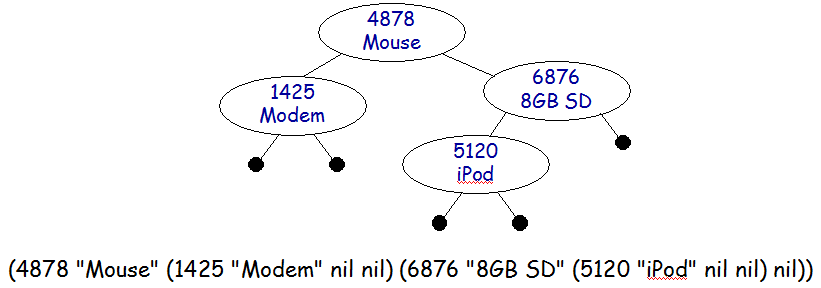
\includegraphics[scale=0.5]{images/searchtree.png}
\end{center}
\caption{Search Tree Diagram and Corresponding Formula}
\label{fig:searchtree-diagram}
\end{figure}

\label{empty-tree}
If the root node is nil, the tree is said to be ``empty''.
\label{subtree}
A ``subtree'' is any part of the tree beginning with a node
and continuing all the way from that node to the leaves.
In a search tree formula, a subtree is a
four-element list (key, data, left subtree, right subtree)
that occurs at some level in the tree structure.
The list could comprise the entire tree or just a portion of it.
Any node represented by nil is also a subtree (an empty one, of course).

Properties of search trees and operations on
them depend on notions such as subtree
and the occurrence of a key in a tree.
Figure \ref{fig:tree-functions} provides formal definitions of these ideas.

\begin{figure}
\begin{center}
\begin{lstlisting}
(defun key (s) (first s))        ; extract root key from s
(defun dat (s) (second s))       ; extract data from s
(defun lft (s) (third s))        ; extract left subtree from s
(defun rgt (s) (fourth s))       ; extract right subtree
(defun emptyp (s) (equal s nil)) ; s is an empty tree
(defun 4-element-list (xs)
  (and (consp xs) (consp (rest xs)) (consp (rest (rest xs)))
       (consp (rest (rest (rest xs))))
       (equal nil (rest (rest (rest (rest xs)))))))
(defun treep (s)                 ; s is a search tree
  (or (emptyp s)
      (and (4-element-list s) (natp (key s))
           (treep (lft s)) (treep (rgt s)))))
(defun subp (r s)                ; r is a subtree of s
  (and (treep r) (treep s)
       (or (emptyp r)
           (and (not (emptyp s))
                (or (subp r (lft s)) (subp r (rgt s)))))))
(defun keyp (k s)                ; key k occurs in s
  (and (not (emptyp s))
       (or (= k (key s)) (keyp k (lft s)) (keyp k (rgt s)))))
\end{lstlisting}
\end{center}
\caption{Search Tree Functions and Predicates}
\label{fig:tree-functions}
\end{figure}

\section{Ordered Search Trees and Tree Induction}

A search tree is ``ordered'' if the key in each non-leaf node is
greater than all the keys that occur in the left subtree of the node
and is less than all the keys that occur in the right subtree. A
leaf is ordered by default. That is, the predicate 
``ordp'' satisfies the following equations.
For any search tree $s$, (ordp $s$) is true if $s$ is ordered 
and false otherwise.

\begin{center}
\begin{tabular}{ll}
(ordp nil) = true  & \{\emph{ord0}\} \\
(ordp (k d lf rt) = ($\forall x$,(keyp $x$ $lf$).$x < k$) $\wedge$
                    ($\forall y$,(keyp $y$ $rt$).$y > k$) $\wedge$
                    (ordp $lf$) $\wedge$  (ordp $rt$) & \{\emph{ord1}\} \\
\end{tabular}
\end{center}

\begin{comment}
From the definition of the predicate ordered, it's not a big step to
guess that an ordered search tree cannot contain duplicate keys.
However, saying exactly what that means turns out to be tricky. One
approach is to define a function that extracts from a search tree a
sequence containing all the data elements in the tree that are
associated with a given key, and then to prove that the sequence
contains exactly one element if the key occurs in an ordered tree.
If the key doesn't occur in the tree, the sequence is empty.\newline

$\ $\newline $\ $\newline

 $\mathbf{sequence}\ \mathbf{of}\  \mathbf{matching}\
\mathbf{keys}$\newline

\begin{verbatim}
dataElems :: SearchTree d -> Integer -> [d]
dataElems Nub x = []                            {dataElems N}
dataElems (Cel k d lf rt) x                     {dataElems C}
  = if k == x
       then (dataElems lf x) ++ [d] ++ (dataElems rt x)
       else (dataElems lf x) ++ (dataElems rt x)
\end{verbatim}

\begin{theorem}
\label{th:uk_1}

(unique keys, part 1).

$\forall s. (\mathit{ordered}\ (s)\  \logand\   \mathtt{k} \in s)\
\logimp\  (\mathtt{length}\ (\mathtt{dataElems}\  s\  \mathtt{k})\
==\  1)$

\end{theorem}

\begin{theorem}
\label{th:uk_2}

(unique keys, part 2).

$\forall s. (\mathit{ordered}\ (s)\  \logand\   \mathtt{k} \not\in
s)\  \logimp\  ((\mathtt{dataElems}\  \mathit{s}\  \mathtt{k})\  ==\
[ ])$

\end{theorem}

We will prove\index{$\mathtt{dataElems}$} Theorem \ref{th:uk_2}
first, and we will use a new form of induction that we will call
{\bf tree induction}\index{tree induction}.

%$$\mathbf{Principle}\  \mathbf{of}\  \mathbf{Tree}\
%\mathbf{Induction}.

\medskip
\noindent\textbf{Principle of Tree Induction.}

$$
  (\forall\  t.\ (\forall\  s\subset t.\  P(s))\
\logimp\  P(t))\ \logimp\  (\forall t.\  P(t))$$

Note: The domain of discourse of the for-alls is the set of all
search trees.

The principle of induction derives from basic elements of set
theory, and all forms of inductive proof are equivalent when taken
back to this basic framework. In practice, the form of induction
used in a particular proof depends on the domain of discourse.
Verifying the equivalence of various inductive forms to ordinary,
mathematical induction on the natural numbers would require a major
digression into details of set theory.



Using the principle of tree induction, we can prove that a predicate
is true for every search tree if we can prove a certain implication.
The implication is this: if the predicate is true for every proper
subtree of a particular, chosen tree, then it must also be true for
the chosen tree. The implication must be proved for an arbitrarily
chosen tree, but once this implication is proved, the principle of
tree induction delivers the conclusion that the predicate is true
for every search tree.

The statement of the principle of tree induction is identical to the
statement of strong induction for the domain of natural numbers,
except that where the relation ``less than'' appears in the
principle of strong induction, the relation ``proper subset''
appears in the principle of tree induction. The two forms of
induction share the implicit requirement that the predicate must be
proved directly for the simplest element.

In the case of strong induction, the simplest element is zero. There
are no natural numbers smaller than zero. Therefore, when the chosen
element is zero, the universe of discourse for the for-all in the
hypothesis of the implication $(\forall\ s < 0.\  P(s))$ is empty. A
for-all over an empty universe of discourse is true by default, so
for the case when the chosen element is zero, the implication to be
proved is $(\True\ \logimp\  P(0))$. The hypothesis in this
implication can be of no help in proving its conclusion.


The same is true for tree induction. When the chosen element is a
$\mathtt{Nub}$, the universe of discourse for the hypothesis of the
implication to be proved is empty. That is, we must prove
$((\forall\ s\subset \mathtt{Nub}.\  P(s))\ \logimp\
P(\mathtt{Nub}))$, which is the same as $(\True\ \logimp\
P(\mathtt{Nub}))$. The hypothesis of this implication (namely,
``true'') cannot help in arriving at its conclusion (namely,
$P(\mathtt{Nub})$). We will use tree induction to prove many
properties of software that operates on search trees, and a few
properties of the search trees themselves. For starters, we use tree
induction to prove Theorem \ref{th:uk_2}.

\begin{proof} of Theorem \ref{th:uk_2}

(unique keys, part 2):

$\forall s. (\mathit{ordered}\ (s)\  \logand\   \mathtt{k} \not\in
s)\  \logimp\  ((\mathtt{dataElems}\  \mathtt{s}\  \mathtt{k})\  ==\
[ ])$\newline

Proof: by tree induction.\newline

Base Case.\newline

$\begin{array}{ll}

(\mathit{ordered}\ (\mathtt{Nub})\  \logand\   \mathtt{k} \not\in

\mathtt{Nub})\ \logimp\ ((\mathtt{dataElems}\  \mathtt{Nub}\

\mathtt{k})\ ==\ [ ]) & \\

\quad =\ \{\mathit{ord}\  N, \in N\} & \\

(\False \ \logand\  \False)\  \logimp\

((\mathtt{dataElems}\  \mathtt{Nub}\  \mathtt{k})\  ==\  [ ]) & \\

\quad =\  \{\logand\  \mathit{idem}\} & \\

\False\ \logimp\   ((\mathtt{dataElems}\  \mathtt{Nub}\  \mathtt{k})

\ ==\  [ ]) & \\

\quad =\ \{\False \ \logimp\ \mathit{any}\  =\ \True\} & \\

\True & \\

\end{array}$\newline

Inductive Case.\newline

First, we work with just the hypothesis of the implication we're
trying to prove.\newline

$\begin{array}{l}

  (\mathit{ordered}\ (\mathtt{Cel}\  \mathtt{x}\  \mathtt{a}\  \mathtt{lf}\

\mathtt{rt})\ \logand\

   \mathtt{k}\ \not\in\  (\mathtt{Cel}\  \mathtt{x}\  \mathtt{a}\

\mathtt{lf}\

   \mathtt{rt})) \\

\quad =\  \{\in\ C\} \\

(\mathit{ordered}\ (\mathtt{Cel}\  \mathtt{x}\  \mathtt{a}\

\mathtt{lf}\  \mathtt{rt})\  \logand\  \lognot (\mathtt{x}\  =\

\mathtt{k}\  \logor\  \mathtt{k} \in \mathtt{lf}\ \logor\ \mathtt{k}

\in \mathtt{rt} )) \\

\quad = \ \{DM\} \\

(\mathit{ordered}\ (\mathtt{Cel}\  \mathtt{x}\  \mathtt{a}\

\mathtt{lf}\  \mathtt{rt})\ \logand\  (\mathtt{x} \not =

\mathtt{k})\ \logand\  (\mathtt{k} \not\in \mathtt{lf})\ \logor\

(\mathtt{k} \not\in \mathtt{rt} )) \\

\end{array}$\newline

We are trying to prove that when the above formula is true, the
formula in the conclusion of the theorem is also true. That is, we
want to prove that the $\mathtt{dataElems}$ function delivers an
empty sequence in this case.\newline

$\begin{array}{l}

\mathtt{dataElems}\  (\mathtt{Cel}\  \mathtt{x}\  \mathtt{a}\


\mathtt{lf}\  \mathtt{rt})\  \mathtt{k} \\





\quad = \ \{\mathtt{dataElems}\  C, \mathtt{x} \not = \mathtt{k}\} \\






(\mathtt{dataElems}\  \mathtt{lf}\  \mathtt{k})\ \append \


(\mathtt{dataElems}\  \mathtt{rt}\  \mathtt{k}) \\





\quad = \ \{\mathit{ord}\  C ,k \not\in \mathtt{lf},


\mathit{induction}\  \mathit{hypothesis},\  \mathit{applied}\


\mathit{twice}\} \\





[ ]\  \append\  [ ] \\





\quad = \ \{\append\ [ ]\} \\





[ ] \\





\end{array}$

The induction step in the proof occurred when we observed that with
respect to the formula $(\mathtt{dataElems}\  \mathtt{lf}\
\mathtt{k})$, the hypotheses of the theorem are true. That is, the
tree $\mathtt{lf}$ is ordered (by the definition of ordered, since
$\mathtt{lf}$ is a subtree of an ordered tree) and the key
$\mathtt{k}$ does not occur in that tree. As $\mathtt{lf}$ is a
proper subtree of the tree we started with, the principle of
induction allows us to assume that the theorem is true for the tree
$\mathtt{lf}$. (Remember, induction doesn't require a direct proof
in the inductive case. It only requires that you prove an
implication whose hypothesis is that the theorem is true for every
proper subtree of the one you started with.) In this case, we apply
the induction hypothesis twice: once for the left subtree and again
for the right subtree.
\end{proof}

Now, what about Theorem \ref{th:uk_1}? Induction also provides the
mechanism for its proof.\newline

%Theorem \ref{th:uk_1} (unique keys, part 1).
%

%$\forall s. (\mathit{ordered}\ (s)\ \logand\   \mathtt{k} \in s)\

%\logimp\  (\mathtt{length}\ (\mathtt{dataElems}\  s\  \mathtt{k})\

%==\  1)$\newline

\begin{proof} of Theorem  \ref{th:uk_1} (unique keys, part 1), by tree
induction.\newline

Base Case.\newline

$\begin{array}{l}

  (\mathit{ordered}\ (\mathtt{Nub})\ \logand\  \mathtt{k}\in \mathtt{Nub})\

\logimp\

  (\mathtt{length}\ (\mathtt{dataElems}\  \mathtt{Nub}\  \mathtt{k})\  =
=\

  1) \\

\quad =\ \{\in N\} \\

(\mathit{ordered}\ (\mathtt{Nub})\  \logand\  \False)\ \logimp\

(\mathtt{length}\ (\mathtt{dataElems}\  \mathtt{Nub}\  \mathtt{k}) \

==\  1) \\

\quad = \ \{\logand\  null\} \\

\False\ \logimp\   (\mathtt{length}\ (\mathtt{dataElems}\

\mathtt{Nub}\  \mathtt{k})\  ==\  1) \\

\quad =\ \{\False \ \logimp\ \mathit{any}\  =\  \True\} \\

\True

\end{array}$\newline

Inductive Case.\newline

First, we work with just the hypothesis of the implication we're
trying to prove.\newline

$\begin{array}{l}





  (\mathit{ordered}\ (\mathtt{Cel}\  \mathtt{x}\  \mathtt{a}\  \mathtt{lf}\



\mathtt{rt})\ \logand\   \mathtt{k} \in


   (\mathtt{Cel}\  \mathtt{x}\  \mathtt{a}\  \mathtt{lf}\  \mathtt{rt})) \\






\quad =\ \{\in C\} \\





(\mathit{ordered}\ (\mathtt{Cel}\  \mathtt{x}\  \mathtt{a}\


\mathtt{lf}\  \mathtt{rt})\  \logand\  (\mathtt{x} = \mathtt{k}\


\logor\ \mathtt{k} \in \mathtt{lf}\ \logor\  \mathtt{k} \in


\mathtt{rt} ))


\\





\quad =\ \{\logand\ \mathit{over}\  \logor\} \\





(\mathit{ordered}\ (\mathtt{Cel}\  \mathtt{x}\  \mathtt{a}\  \mathtt{lf}\



\mathtt{rt})\   \logand\


  (\mathtt{x} = \mathtt{k}))\   \logor\   \\





   (\mathit{ordered}\ (\mathtt{Cel}\  \mathtt{x}\  \mathtt{a}\  \mathtt{lf}
\


  \mathtt{rt})\   \logand\


   \mathtt{k} \in \mathtt{lf})\   \logor\  \\


   (\mathit{ordered}\ (\mathtt{Cel}\  \mathtt{x}\  \mathtt{a}\  \mathtt{lf}
\


  \mathtt{rt})\   \logand


   \mathtt{k} \in \mathtt{rt}) \\


\end{array}$\newline

We are trying to prove that when the above formula is true, the
formula in the conclusion of the theorem is also true. That is, we
want to prove that the $\mathtt{dataElems}$ function delivers a
sequence with exactly one element in this case. The implication we
are trying to verify has the following form: $(a\  \logor\  b\
\logor\  c)\ \logimp\  d$, where $d$ is the conclusion of the
theorem (that is, $d\  =\  (\mathtt{length}\ (\mathtt{dataElems}\ s\
\mathtt{k})\  ==\  1))$, and $a$, $b$, and $c$ are the terms in the
above formula. For example, $a\  =\  (\mathit{ordered}\
(\mathtt{Cel}\  \mathtt{x}\  \mathtt{a}\  \mathtt{lf}\ \mathtt{rt})\
\logand\  (\mathtt{x}\  =\  \mathtt{k}))$. Using the Boolean algebra
of propositions, one can verify that

$((a\  \logor\  b\  \logor\  c)\ \logimp\  d)\  =\  ((a\  \logimp\
d)\ \logand\  (b\  \logimp\  d)\ \logand\ (c\  \logimp\  d))$

That is, the formula $((a\  \logor\  b\  \logor\  c)\  \logimp\  d)$
can be verified by proving that each of the terms, $(a\  \logimp\
d)$, $(b\ \logimp\  d)$, and $(c\ \logimp\  d)$, is true.\newline

Proof of $(a\ \logimp\  d)$:

$(\mathit{ordered}\ (\mathtt{Cel}\  \mathtt{x}\  \mathtt{a}\
\mathtt{lf}\ \mathtt{rt})\  \logand\ (\mathtt{x}\  =\  \mathtt{k}))\
\logimp\ $

$\quad\quad\quad(\mathtt{length}\ (\mathtt{dataElems}\
(\mathtt{Cel}\ \mathtt{x}\ \mathtt{a}\  \mathtt{lf}\  \mathtt{rt})\
\mathtt{k})\ ==\  1)$

Again, we work with the hypothesis of the implication first. Since
the tree $(\mathtt{Cel}\  \mathtt{x}\  \mathtt{a}\  \mathtt{lf}\
\mathtt{rt})$ is ordered, $\mathtt{x} \not\in \mathtt{lf}$ and
$\mathtt{x} \not\in \mathtt{rt}$. (All the keys in the left subtree
must be smaller than $\mathtt{x}$, and all those in the right
subtree must be larger than $\mathtt{x}$. Because $\mathtt{x}\  =
\mathtt{k}$, we conclude that $\mathtt{k} \not\in \mathtt{lf}$ and
$\mathtt{k} \not\in \mathtt{rt}$.) These observations take us to the
conclusion of the theorem by the following logic.\newline

$\begin{array}{l}
\mathtt{length}\ (\mathtt{dataElems}\
(\mathtt{Cel}\  \mathtt{x}\


\mathtt{a}\ \mathtt{lf}\  \mathtt{rt})\  \mathtt{k}) \\

\quad = \ \{\mathtt{dataElems}\  C, \mathtt{x}\  =\  \mathtt{k}\} \\

\mathtt{length}\ ((\mathtt{dataElems}\  \mathtt{lf}\  \mathtt{k})\
\append\

[\mathtt{a}]

\  \append\  (\mathtt{dataElems}\  \mathtt{rt}\  \mathtt{k})) \\

\quad = \ \{\mathit{Thm}\ \ref{th:uk_2}, \mathtt{k}\ \not\in
\mathtt{lf}\}

\\

\mathtt{length}\ ([ ]\  \append  [\mathtt{a}]\  \append\

(\mathtt{dataElems}\  \mathtt{rt}\  \mathtt{k}))    \\

\quad =\  \{\mathit{Thm}\ \ref{th:uk_2}, \mathtt{k}\ \not\in
\mathtt{rt}\}

\\

\mathtt{length}\ ([ ]\  \append\  [\mathtt{a}]\  \append\  [ ])     \\

\quad =\ \{\append.1, \append []\} \\

\mathtt{length}\ ([\mathtt{a}])   \\

\quad = \ \{\mathit{Thm}\  \mathit{len}\} \\

1     \\

\end{array}$\newline

It turns out that the induction hypothesis was not needed for the
proof of $(a\  \logimp\  d)$. It will be needed for the other two
proofs, however.\newline

Proof of $(b\  \logimp\  d)$:

$\begin{array}{l}
(\mathit{ordered}\ (\mathtt{Cel}\  \mathtt{x}\  \mathtt{a}\  \mathtt{lf}\
\mathtt{rt})\ \logand\   \mathtt{k} \in \mathtt{lf})\  \logimp\
\\
\qquad (\mathtt{length}\ (\mathtt{dataElems}\  (\mathtt{Cel}\  \mathtt{x}\
\mathtt{a}\ \mathtt{lf}\  \mathtt{rt})\   \mathtt{k})\  ==\  1)
\end{array}$

Again, we work with the hypothesis of the implication first.

$\begin{array}{l}

  (\mathit{ordered}\ (\mathtt{Cel}\  \mathtt{x}\  \mathtt{a}\  \mathtt{lf}\



\mathtt{rt})\


\logand\   \mathtt{k} \in \mathtt{lf}) \\





\quad \logimp\ \{\mathit{definition}\  \mathit{of}\  \mathit{ordered}\} \\






(\mathit{ordered}\ (\mathtt{Cel}\  \mathtt{x}\  \mathtt{a}\


\mathtt{lf}\ \mathtt{rt})\


\logand\   \mathtt{k} \in \mathtt{lf}\ \logand\ \mathtt{k} < \mathtt{x}) \\






\quad \logimp\ \{\mathit{def}\


\mathit{ord}, \mathit{since}\


\mathtt{k} < \mathtt{x}\


\logimp\


\mathtt{k} \not\in \mathtt{rt}\}\


\\





(\mathit{ordered}\ (\mathtt{Cel}\  \mathtt{x}\  \mathtt{a}\


\mathtt{lf}\ \mathtt{rt})\


\logand\   \mathtt{k} \in \mathtt{lf}\ \logand\ \mathtt{k} < \mathtt{x}\



\logand\ \mathtt{k} \not\in


\mathtt{rt}) \\





%(\mathit{ordered}\ (\mathtt{Cel}\  \mathtt{x}\  \mathtt{a}\


%\mathtt{lf}\  \mathtt{rt})\ \logand\  \mathtt{k} \in \mathtt{lf}\


%\logand\  \mathtt{k} < \mathtt{x}\ \logand\   \mathtt{k} \not\in


%\mathtt{rt}) \\





\quad \logimp\ \{\mathtt{dataElems}\  C, \mathtt{k} < \mathtt{x}\} \\





((\mathtt{dataElems}\  (\mathtt{Cel}\  \mathtt{x}\  \mathtt{a}\


\mathtt{lf}\  \mathtt{rt})\  \mathtt{k})\  =\ \\

 \qquad  (\mathtt{dataElems}\


\mathtt{lf}\  \mathtt{k})\  \append\  (\mathtt{dataElems}\  \mathtt{rt}\



\mathtt{k})) \\





        \logand\   (\mathit{ordered}\ (\mathtt{Cel}\  \mathtt{x}\


\mathtt{a}\  \mathtt{lf}\  \mathtt{rt})\


        \logand\   \mathtt{k} \in \mathtt{lf}\   \logand\   \mathtt{k}



\not\in \mathtt{rt})\\





\quad \logimp\ \{\mathit{Thm}\  \ref{th:uk_2}\} \\





((\mathtt{dataElems}\  (\mathtt{Cel}\  \mathtt{x}\  \mathtt{a}\


\mathtt{lf}\  \mathtt{rt})\  \mathtt{k})\  =\  (\mathtt{dataElems}\


\mathtt{lf}\  \mathtt{k})\  \append\  []) \\





        \logand\   (\mathit{ordered}\ (\mathtt{Cel}\  \mathtt{x}\


\mathtt{a}\  \mathtt{lf}\  \mathtt{rt})\


        \logand\   \mathtt{k} \in \mathtt{lf}\   \logand\   \mathtt{k}



\not\in \mathtt{rt})\\





\quad \logimp\ \{\append\ [ ]\} \\





((\mathtt{dataElems}\  (\mathtt{Cel}\  \mathtt{x}\  \mathtt{a}\


\mathtt{lf}\  \mathtt{rt})\  \mathtt{k})\  =\  (\mathtt{dataElems}\


\mathtt{lf}\  \mathtt{k})) \\





        \logand\   (\mathit{ordered}\ (\mathtt{Cel}\  \mathtt{x}\


\mathtt{a}\  \mathtt{lf}\  \mathtt{rt})\


        \logand\   \mathtt{k} \in \mathtt{lf}\   \logand\   \mathtt{k}



\not\in \mathtt{rt})\\





\end{array}$\newline

Now, because $\mathtt{lf}$ is a subtree of $(\mathtt{Cel}\ \mathtt{x}\
\mathtt{a}\  \mathtt{lf}\  \mathtt{rt})$, $\mathtt{k} \in
\mathtt{lf}$, and $\mathtt{lf}$ is ordered, the induction hypothesis
leads to the desired conclusion.

\medskip
$\begin{array}{l}
$$\mathtt{length}\ (\mathtt{dataElems}\ (\mathtt{Cel}\  \mathtt{x}\
\mathtt{a}\  \mathtt{lf}\  \mathtt{rt})\ \mathtt{k})\  \\
 \qquad =\
\mathtt{length}\ (\mathtt{dataElems}\ \mathtt{lf}\ \mathtt{k})\  \\
 \qquad \qquad =\
1\ \ \{\mathit{induction}\  \mathit{hypothesis}\}
\end{array}$
\medskip

The proof of $(c \ \logimp\  d)$ is similar to the proof of $(b \
\logimp\ d)$, except that the induction goes down the right side of
the tree instead of the left.
\end{proof}

\subsection{Retrieving Data from a Search Tree}

According to Theorem \ref{th:uk_1}, a key that occurs in an ordered
search tree occurs exactly once. It occurs as one of the parameters
of a $\mathtt{Cel}$ constructor, and that constructor will also have
a data item as a parameter. Retrieving data from an ordered search
tree amounts to finding the $\mathtt{Cel}$ constructor where a
specified key occurs, then delivering the data item from that same
$\mathtt{Cel}$ constructor.

The retrieval operation needs a way to signal whether or not the
specified key is present in the tree. In our implementation, this
will be done using the $\mathtt{Maybe}$ data type, which has two
constructors: $\mathtt{Just}$ and $\mathtt{Nothing}$. The
$\mathtt{Just}$ constructor will be used to deliver the data item
associated with the given key in the tree. For example,
$(\mathtt{Just}\  \mathtt{d})$ delivers the data item $\mathtt{d}$.

If the key is not present, the $\mathtt{Nothing}$ constructor will
be used to signal that it is missing. So, if the retrieval function
delivers $\mathtt{Nothing}$, the specified key is not present in the
tree.

\begin{verbatim}
getItem :: SearchTree d -> Integer -> Maybe d
getItem (Cel k d lf rt) x  =
  if x < k
      then (getItem lf x)
      else if x > k then (getItem rt x)
      else (Just d)
getItem Nub x = Nothing
\end{verbatim}

We can conclude that $\mathtt{getItem}$\index{$\mathtt{getItem}$}
works properly if we can prove that whenever the key specified in
its second argument is present in the tree given in its first
argument, then $\mathtt{getItem}$ delivers the data item associated
with that key and that if the key is not present, $\mathtt{getItem}$
delivers $\mathtt{Nothing}$. We will use tree induction to prove
both of these facts.

\begin{theorem}


\label{th:getItem_1}

$\forall s. (\mathit{ordered}\ (s)\   \logand\   \mathtt{k} \in s)\
\logimp\  ((\mathtt{getItem}\  s\  \mathtt{k})\  =\ (\mathtt{Just}\
\mathtt{d}))$, where $\mathtt{d}$ is the data item parameter of the
$\mathtt{Cel}$ constructor in $s$ for which $\mathtt{k}$ is the key
parameter.


\end{theorem}

\begin{proof}

$$ (\mathtt{k} \in  s)\  \logimp\  (s\  =\  (\mathtt{Cel}\  \mathtt{x}\
\mathtt{a}\  \mathtt{lf}\  \mathtt{rt}))\  \logand\  ((\mathtt{k}\
=\ \mathtt{x})\ \logor\  \mathtt{k} \in \mathtt{lf} \   \logor\
\mathtt{k} \in \mathtt{rt}) \quad\quad\quad \{\in C\}$$

Now we are in the same situation as in the proof of Theorem
\ref{th:uk_1} (not surprising, as the hypotheses\index{$(\in C)$}
of Theorem \ref{th:getItem_1} are the same as those of Theorem
\ref{th:uk_1}). We want to prove an implication whose hypothesis is
a three-way disjunction. We follow the same strategy: separate the
implication into a conjunction of three implications, and prove each
of them separately.

\begin{enumerate}


\item


Proof of


$(\mathit{ordered}\ (\mathtt{Cel}\  \mathtt{x}\  \mathtt{a}\
\mathtt{lf}\  \mathtt{rt})\  \logand\   \mathtt{k} \in
(\mathtt{Cel}\ \mathtt{x}\  \mathtt{a}\ \mathtt{lf}\  \mathtt{rt})\
\logand\   (\mathtt{k}\  =\ \mathtt{x}))\ \logimp\ $


                                                       $((\mathtt{getItem}\
(\mathtt{Cel}\  \mathtt{x}\  \mathtt{a}\  \mathtt{lf}\ \mathtt{rt})\
\mathtt{k})\  =\ (\mathtt{Just}\ \mathtt{d}))$

where $\mathtt{d}$ is the data item parameter of the $\mathtt{Cel}$
constructor in the tree $(\mathtt{Cel}\  \mathtt{x}\ \mathtt{a}\
\mathtt{lf}\  \mathtt{rt})$ for which $\mathtt{k}$ is the key
parameter.

$\begin{array}{l}

(\mathtt{getItem}\  (\mathtt{Cel}\  \mathtt{x}\  \mathtt{a}\


\mathtt{lf}\  \mathtt{rt})\  \mathtt{k} \\





\quad = \ \{\mathtt{k}\  =\  \mathtt{x}\} \\








(\mathtt{getItem}\  (\mathtt{Cel}\  \mathtt{k}\  \mathtt{a}\


\mathtt{lf}\  \mathtt{rt})\  \mathtt{k} \\





\quad = \ \{\mathtt{getItem}\  C\} \\





(\mathtt{Just}\  \mathtt{a)} \\





\end{array}$

Since $\mathtt{a}$ is the data item parameter of the $\mathtt{Cel}$
constructor in the tree $(\mathtt{Cel}\  \mathtt{x}\ \mathtt{a}\
\mathtt{lf}\  \mathtt{rt})$ for which $\mathtt{k}\  =\ \mathtt{x}$
is the key parameter, the desired conclusion has been reached.


\item


Proof of

$(\mathit{ordered}\ (\mathtt{Cel}\  \mathtt{x}\ \mathtt{a}\
\mathtt{lf}\  \mathtt{rt})\ \logand\   \mathtt{k} \in (\mathtt{Cel}\
\mathtt{x}\  \mathtt{a}\  \mathtt{lf}\  \mathtt{rt})\ \logand\
(\mathtt{k} \in \mathtt{lf}))\  \logimp$





$((\mathtt{getItem}\  (\mathtt{Cel}\  \mathtt{x}\ \mathtt{a}\
\mathtt{lf}\ \mathtt{rt})\  \mathtt{k})\  =\  (\mathtt{Just}\
\mathtt{d}))$

where $\mathtt{d}$ is the data item parameter of the $\mathtt{Cel}$
constructor in the tree $(\mathtt{Cel}\  \mathtt{x}\ \mathtt{a}\
\mathtt{lf}\  \mathtt{rt})$ for which $\mathtt{k}$ is the key
parameter.

$\begin{array}{ll}





  (\mathit{ordered}\ (\mathtt{Cel}\  \mathtt{x}\  \mathtt{a}\  \mathtt{lf}\ \mathtt{rt})\   \logand \   \mathtt{k} \in (\mathtt{Cel}\
\mathtt{x}\



\mathtt{a}\  \mathtt{lf}\  \mathtt{rt})


   \   \logand\   (\mathtt{k} \in \mathtt{lf})) & \\





\quad = \ \{\mathit{def}\  \mathit{ordered}\} \\





(\mathit{ordered}\ (\mathtt{Cel}\  \mathtt{x}\ \mathtt{a}\
\mathtt{lf}\ \mathtt{rt})\   \logand \   \mathtt{k} \in
(\mathtt{Cel}\ \mathtt{x}\ \mathtt{a}\  \mathtt{lf}\  \mathtt{rt})


   \   \logand\   (\mathtt{k} < \mathtt{x})) & \\








\quad \logimp \ \{\mathtt{getItem}\ C\} \\





((\mathtt{getItem}\ (\mathtt{Cel}\  \mathtt{x}\  \mathtt{a}\
\mathtt{lf}\ \mathtt{rt})\ \mathtt{k})\ =\ (\mathtt{getItem}\
\mathtt{lf}\ \mathtt{k}))\\





\quad = \ \{\mathit{induction}\ \mathit{hypothesis}\} \\








((\mathtt{getItem}\ (\mathtt{Cel}\  \mathtt{x}\ \mathtt{a}\
\mathtt{lf}\ \mathtt{rt})\ \mathtt{k})\ =\ (\mathtt{Just}\
\mathtt{d}))\\
\end{array}$\newline
where $\mathtt{d}$ is the data item parameter of the $\mathtt{Cel}$
constructor in the tree $(\mathtt{Cel}\  \mathtt{x}\ \mathtt{a}\
\mathtt{lf}\ \mathtt{rt})$ for which $\mathtt{k}$ is the key
parameter.

\item The proof of the third implication required by the three-part
  disjunction is like this last proof, except that the induction
  goes down the right-hand side of the tree instead of the left.
\end{enumerate}

\end{proof}

\subsection{Search Time in the Equational Model}

We can use the equations for $\mathtt{getItem}$ as a prescription
for computation. To compute the value represented by a formula
involving $\mathtt{getItem}$, we simply scan the formula for
subformulas that match the left-hand side of one of the equations.
When we find a match, we replace the subformula by the right-hand
side of the equation (with appropriate substitutions for the
parameters), and we continue this procedure until no subformulas
match the left-hand side of either equation. This procedure of
repeated substitution for subformulas is the {\bf equational model
of computation}\index{equational model of computation}.

If we want to figure out how many computational steps the
equational model of computation requires to deliver the value of a
formula, we count the process of matching a formula with an
equation as a single computational step. We also count any use of
an intrinsic operator, such as logical {\it and} $(\logand)$,
if-then-else selection, the $\mathtt{Just}$ and $\mathtt{Nothing}$
constructors, and the like, as computational steps.

Consider the computation of
the formula $(\mathtt{getItem}\ \mathtt{s}\ \mathtt{k})$.  At each
step, the
equations either deliver the value directly, requiring only the
computational step of matching the formula with the second equation
(this occurs if $\mathtt{s}$ is $\mathtt{Nub}$), or the formula is
replaced by an if-then-else selection. In the latter case, the
process of matching the formula with the first equation counts as
one computational step, and the if-then-else selection counts as
another computational step.

In the case in which the first equation is the one that matches,
the tree $\mathtt{s}$ must have the form $(\mathtt{Cel}\
\mathtt{x}\ \mathtt{a}\ \mathtt{lf}\ \mathtt{rt})$, and the
matching subformula is replaced by the if-then-else selection on
the right-hand side of the equation. Where the computation goes
after this substitution depends on the result of the test in the
if-then-else selection. If $\mathtt{k}$, the key specified in
$(\mathtt{getItem}\ \mathtt{s}\ \mathtt{k})$, is less than
$\mathtt{x}$ (the key in $(\mathtt{Cel}\ \mathtt{x}\ \mathtt{a}\
\mathtt{lf}\ \mathtt{rt})$, which constructs the tree
$\mathtt{s}$), the formula $(\mathtt{getItem}\ \mathtt{s}\
\mathtt{k})$ is replaced by $(\mathtt{getItem}\ \mathtt{lf}\
\mathtt{k})$, and the computation proceeds from there by again
figuring out whether that formula matches the first equation or the
second equation. So, the number of computational steps will be one
for matching the formula $(\mathtt{getItem}\ \mathtt{s}\
\mathtt{k})$ to the first equation, plus one step for the
if-then-else selection, plus the number of steps it takes to
compute $(\mathtt{getItem}\ \mathtt{lf}\ \mathtt{k})$.

On the other hand, if the tree $\mathtt{s}$ has the form
$(\mathtt{Cel}\  \mathtt{x}\  \mathtt{a}\ \mathtt{lf}\ \mathtt{rt})$
and $\mathtt{k}$ is greater than $\mathtt{x}$, then the computation
requires one step to match the first equation, plus one step for the
if-then-else selection that finds out that $(\mathtt{k} <
\mathtt{x})$ is false, plus one step for the if-then else selection
that finds out that $(\mathtt{k} > \mathtt{x})$ is true, plus the
number of steps required to compute $(\mathtt{getItem}\ \mathtt{rt}\
\mathtt{k})$.

Finally, if $\mathtt{k}$ is the same as $\mathtt{x}$, then the
computation requires one step to match the first equation, plus one
for the if-then-else selection that finds out that $(\mathtt{k} <
\mathtt{x})$ is false, plus one for the if-then else selection that
finds out that $(\mathtt{k} > \mathtt{x})$ is false, plus one to
construct the result $(\mathtt{Just}\  \mathtt{a})$.

If we let the symbol $\mathit{gSteps}\ (\mathtt{s}, \mathtt{k})$
stand for the number of computational \index{$\mathit{gSteps}$}steps
required to compute the value represented by the formula
$(\mathtt{getItem}\ \mathtt{s}\ \mathtt{k})$, the above reasoning
leads us to the following numerical relationships:

$\begin{array}{ll}





\mathit{gSteps}\ (\mathtt{Nub}, \mathtt{k})\  =\  1 & \{\mathit{gSteps}\ N\} \\





\mathit{gSteps}\ (\mathtt{Cel}\  \mathtt{x}\ \mathtt{a}\
\mathtt{lf}\  \mathtt{rt}, \mathtt{k})\  \leq\ & \{\mathit{gSteps}\ C\} \\





\mathit{max}\ (\mathit{gSteps}\ (\mathtt{lf}, \mathtt{k})\  +\  2,\


\mathit{gSteps}\ (\mathtt{rt}, \mathtt{k})\  +\  3,4) &  \\





\end{array}$\newline

The important point to notice is either the computation is complete
in one step (if the tree is $\mathtt{Nub})$, or in four steps (if
$\mathtt{k}\  ==\  \mathtt{x})$, or in no more than three more than
the number of steps required to search for $\mathtt{k}$ in a proper
subtree of $\mathtt{s}$. Since the proper subtree is ``shorter''
than the tree the search started with, the number of steps remaining
in the computation is reduced at each stage. Therefore, the total
number of steps will be a sum with one term for each stage in the
computation, and the number of stages in the computation will not
exceed the ``height'' of the tree.

To turn this informal idea into a sound mathematical analysis, we
need to say what we mean by the height\index{height} of a tree. The
idea is that the height of a tree is the longest route from the root
through the subtrees to a $\mathtt{Nub}$. That means that the height
of a tree of the form $(\mathtt{Cel}\  \mathtt{k}\  \mathtt{d}\
\mathtt{lf}\ \mathtt{rt})$ is one more than the height of the taller
of the two subtrees, $\mathtt{lf}$ and $\mathtt{rt}$.  Here are some
equations the height measurement satisfies:

\begin{verbatim}
height :: SearchTree d -> Integer
height Nub = 0                               {height N}
height(Cel kd lf rt) =
   1 + (max (height lf) (height rt))         {height C}
\end{verbatim}

From these equations, it follows that the height of every tree is
non-negative. This fact can be guessed from the observation that
height is computed by adding non-negative numbers to zero and can be
proved by tree induction. In the same vein, it follows that
$\mathit{gSteps}\ (s)$ is non-negative. We are going to imagine that
we have carried out a proof of Theorem \ref{th:height_1}.

\begin{theorem}


\label{th:height_1}

$\forall s.\ \mathtt{height}\ (s)\  \geq\  0$

We reasoned informally that the number of computation steps required
to retrieve a data item from a tree is a sum whose number of terms
is the height of the tree. It turns out that each of the terms in
that sum is about the same size. Therefore, the number of steps in
retrieval is proportional to the height of the tree. Theorem
\ref{th:height_2} makes this notion precise. We will use tree
induction to prove it.


\end{theorem}


\begin{theorem}


\label{th:height_2}





$\forall s.\ \forall k.\  \mathit{gSteps}\ (s, k)\ \leq \ 4\ *\
(\mathtt{height}\ (s)\  +\  1)$


\end{theorem}





\begin{proof}


By tree induction.

Base Case.\newline

$\begin{array}{ll}





\mathit{gSteps}\ (\mathtt{Nub}, \mathtt{k}) & \\





\quad =\ \{\mathit{gSteps}\  N\} \\





1 & \\





\quad \leq\    \{\mathit{arithmetic}\} \\





4\ *\ (0\  +\  1) & \\





\quad =\ \{\mathtt{height}\ N\} \\





4\ *\ (\mathtt{height}\ (\mathtt{Nub})\  +\  1) &\\


\end{array}$\newline





Inductive Case.\newline





$\begin{array}{l}





\mathit{gSteps}\ (\mathtt{Cel}\  \mathtt{x}\  \mathtt{a}\


\mathtt{lf}\  \mathtt{rt},\  \mathtt{k})  \\





\quad \leq\ \{\mathit{gSteps}\  C\} \\





\mathit{max}\ (2\  +\  \mathit{gSteps}\ (\mathtt{lf}, \mathtt{k}),


3\ +\  \mathit{gSteps}\ (\mathtt{rt}, \mathtt{k}), 4) \\





\quad \leq\ \{\mathit{induction}\


\mathit{hypothesis},\  \mathit{applied}\  \mathit{twice}\} \\





\mathit{max}\ (4\ *\ (\mathtt{height}\ (\mathtt{lf})\  +\  1)\  +\


2,\  4\ *\ (\mathtt{height}\ (\mathtt{rt})\  +\


1)\  +\  3,\  4)  \\





\quad \leq \ \{\mathit{arithmetic}\} \\





\mathit{max}\ (4\ *\ (\mathtt{height}\ (\mathtt{lf})\  +\  1)\  +\


4,\  4\ *\ (\mathtt{height}\ (\mathtt{rt})\  +\


1)\  +\  4,\  4)  \\





\quad \leq \ \{\mathit{Thm}\ \ref{th:height_1},\ \mathit{arithmetic}\}\\





\mathit{max}\ (4\ *\ (\mathtt{height}\ (\mathtt{lf})\  +\  1)\ +\
4,\  4\ *\ (\mathtt{height}\ (\mathtt{rt})\  +\ 1)\  +\  4)  \\





\quad =\ \{\mathit{arithmetic}\}\\





4\ *\ \mathit{max}\ ((\mathtt{height}\ (\mathtt{lf})\  +\  1)\  +\  1,\



(\mathtt{height}\ (\mathtt{rt})\  +\


1)\  +\  1)   \\





\quad =\ \{\mathit{arithmetic}\}\\





4\ *\ ((\mathit{max}\ (\mathtt{height}\ (\mathtt{lf}),\  \mathtt{height}\



(\mathtt{rt}))\  +\  1)\  +\  1)  \\





\quad =\ \{\mathit{arithmetic}\}\\





4\ *\ ((1\ +\ \mathit{max}\ (\mathtt{height}\ (\mathtt{lf}),\


\mathtt{height}\ (\mathtt{rt})))\  +\  1)  \\





\quad =\ \{\mathtt{height}\ C\}\\





4\ *\ (\mathtt{height}\ (\mathtt{Cel}\  \mathtt{x}\  \mathtt{a}\


\mathtt{lf}\  \mathtt{rt})\  +\  1) \\





\end{array}$\newline





\end{proof}

Theorem \ref{th:height_2} guarantees that retrieval time will be
short, even for trees that contain a very large number of data
items, as long as the tree has a compact shape (not too tall,
compared to the number of data items in the tree). In the most
compact trees, the number of data items doubles every time the
height increases by one. For example, a tree of height one must have
the form $(\mathtt{Cel}\  \mathtt{k}\  \mathtt{d}\ \mathtt{Nub}\
\mathtt{Nub})$. This tree contains exactly one data item. We can add
data items to this tree by replacing its two subtrees by trees that
contain a data item. The new tree would have height two and contain
three data items. It would look like this:

$$(\mathtt{Cel}\  \mathtt{k}\  \mathtt{d}\  (\mathtt{Cel}\  \mathtt{x}\ \mathtt{a}\  \mathtt{Nub}\ \mathtt{Nub})\  (\mathtt{Cel}\  \mathtt{y}\  \mathtt{b}\
\mathtt{Nub}\ \mathtt{Nub})).$$

Now the two subtrees, $(\mathtt{Cel}\ \mathtt{x}\ \mathtt{a}\
\mathtt{Nub}\ \mathtt{Nub})$ and $(\mathtt{Cel}\ \mathtt{y}\
\mathtt{b}\ \mathtt{Nub}\ \mathtt{Nub})$ can be modified in the
same way to build a tree of height three with seven data items. It
is possible to prove, by ordinary mathematical induction, that a
tree of height $n$ constructed by this procedure contains $2^n-1$
data items.

Trees containing a number of data items falling between the gaps in
the sequence $1, 3, 7,\ldots 2^n-1,\ldots$ can be constructed by
leaving out some of the data items on the most interior level.


Following this pattern, it is possible to put $n$ data items in a
tree of height $\mathit{log}_2(n)$. For trees constructed in a shape
like this, the retrieval time required by the $\mathtt{getItem}$
function becomes relatively shorter (relative, that is, to the
number of data items in the tree) as the number of data items
increases. It is this fact that makes it possible for retrieval of
data in trees to be way faster than retrieval of unordered data from
array-like structures, such as rows of filing cabinets. For a
million items in a compact tree, retrieval, according to Theorem
\ref{th:height_2}, takes no more than $4\ *\ (\mathit{log}_2\
1,000,000\  +\  1)$, which is about 80 steps. Compare this to about
500,000 steps, on the average, to retrieve an item from an unordered
array.

On the other hand, retrieval from data arranged in order in an array
can be as fast as retrieval from a compact tree. However, the number
of steps required to insert or delete an item from an ordered array
is, on the average, proportional to the number of items stored in
the array. If there are a million items in the array, arranged in
increasing order, inserting a new one in the middle will require, on
the average, moving the half-a-million-or-so items beyond the
insertion point. There is room for lots of improvement in the
average speed of insertion. It turns out that insertion and deletion
in a search tree can be accomplished in an amount of time that
increases at the same rate as the height of the tree.

In other words, insertion and deletion in search trees can be done
as efficiently as retrieval. It's not easy to figure out how to do
this. The rest of this chapter is devoted to explaining the AVL
method of efficient insertion and deletion in search trees.

\section{Balanced Trees}

Retrieval, insertion, and deletion in a search tree can be done in
an amount of time proportional to the height of the tree. Therefore,
it is important to keep a lid on height as items are added or
deleted from the tree. The height of a search tree must grow at
least as fast as the logarithm of the number of data items in the
tree (another fact that can be proved by induction). Height will
grow faster than the logarithm of the number of data items unless
the two sides of the tree, left and right, remain balanced as items
are inserted.

When we discussed constructing a tree whose height was proportional
to the logarithm of the number of data items it contained, we were
careful, at each stage, to put the same number of items in the
left-hand side of the tree as in the right-hand side. This is known
as node balancing\index{node balancing}. It is the most
straightforward way to maintain enough balance to keep a tight lid
on height as nodes are inserted, but it turns out to be expensive
to maintain node-balancing in trees as items are inserted.

Another form of balancing, known as height balancing, is cheaper to
accomplish. Fortunately, height-balanced trees also have the
property that height grows at the same rate as the logarithm of the
number of data items. This makes it possible to carry out retrieval,
insertion, and deletion efficiently. A tree is height balanced if,
at all levels, the height of the left subtree is either the same as
the height of the right subtree, or taller by one, or shorter by
one. This notion is made precise by the following
definition\index{$\mathit{balanced}$}.

\medskip
$\begin{array}{l}
$$\mathit{balanced}\ (s)\  =\  \hspace{7cm}\{\mathit{bal}\} \\
  \qquad \forall\ (\mathtt{Cel}\  \mathtt{k}\ \mathtt{d}\  \mathtt{lf}\  \mathtt{rt})
\subseteq\  s.\  \vert\ \mathtt{height}\ (\mathtt{lf})\ -\
\mathtt{height} \ (\mathtt{rt})\ \vert\  \leq\  1
\end{array}$
\medskip


\begin{figure}
\begin{center}
\includegraphics[scale=0.5]{figures/avl-fig2.eps}
\end{center}
\caption{Diagram of Height Balanced Search Tree}
\label{fig:Figure_2}
\end{figure}

Figure \ref{fig:Figure_2} displays a height balanced tree, and
Figure \ref{fig:Figure_3} displays a tree that is not height
balanced. Neither tree is node balanced.

Our goal is to define an insertion operator that preserves order,
balance, and the items in the tree. That is, we want the insertion
operator, for which we use the symbol $(\hatcolon)$, to satisfy the
following properties.

$\begin{array}{lr}

 \quad\ \forall \mathtt{s}.\  \forall \mathtt{k}.\
\forall


\mathtt{d}.\ \mathit{ordered}\ (\mathtt{s})\ \logimp \


\mathit{ordered}\ ((\mathtt{k},\


\mathtt{d})\  \hatcolon\  \mathtt{s}) & \{\hatcolon\ \mathit{ord}\} \\
\quad\ \forall \mathtt{s}.\  \forall \mathtt{k}. \
\forall\mathtt{d}.\ \mathit{balanced}\ (\mathtt{s})\ \logimp \
\mathit{balanced}
\ ((\mathtt{k},\ \mathtt{d})\  \hatcolon\  \mathtt{s}) & \{\hatcolon\ \mathit{bal}\}\\





\quad\ \forall \mathtt{s}.\  \forall \mathtt{k}.\  \forall


\mathtt{d}.\ \forall \mathtt{x}.\ (\mathtt{x} \in \mathtt{s})\
\logimp\  (\mathtt{x} \in ((\mathtt{k}, \mathtt{d}) \hatcolon


\mathtt{s}))& \{\hatcolon \mathit{old}\in\} \\





\quad\ \forall \mathtt{s}.\  \forall \mathtt{k}.\  \forall


\mathtt{d}.\ \mathtt{k} \in ((\mathtt{k}, \mathtt{d}) \hatcolon


\mathtt{s})& \{\hatcolon \mathit{new}\in\} \\





\quad\ \forall \mathtt{s}.\  \forall \mathtt{k}.\  \forall


\mathtt{d}.\ \forall \mathtt{x}.\ ((\mathtt{x} \not\in \mathtt{s})\


\logand\ (\mathtt{x}\ \not =\ \mathtt{k})) \logimp\  (\mathtt{x}


\not\in ((\mathtt{k}, \mathtt{d}) \hatcolon \mathtt{s})) &


\{\hatcolon \not\in\} \\





\end{array}$

Furthermore, the number of steps required to carry out an insertion
must grow in the same proportion as the height of the
\index{$\hatcolon\ \mathit{ord}$}\index{$\hatcolon\
\mathit{bal}$}\index{$\hatcolon \mathit{old}\in$}\index{$\hatcolon
\mathit{new}\in$}\index{$\hatcolon \not\in$}tree.

\begin{figure}
\begin{center}
\includegraphics[scale=0.5]{figures/avl-fig3.eps}
\end{center}
\caption{Diagram of Unbalanced Search Tree}
\label{fig:Figure_3}
\end{figure}

It is not difficult to find ways to insert new items into small
search trees, while maintaining order and balance. To preserve
order, simply find the place at the most interior part of the tree
where the new key goes, moving left or right down the tree according
to whether the new key is smaller or larger than the key being
considered. When you arrive at a $\mathtt{Nub}$, replace it with a
$\mathtt{Cel}$- constructed tree containing the new key, its
associated data, and two $\mathtt{Nub}$ subtrees. This automatically
preserves order. If you're lucky, it may also preserve balance.
However, the replacement subtree has height 1, while the subtree it
replaced (a $\mathtt{Nub}$ tree) had height zero. If this happens to
occur at a point where the tree was already tall, this can make it
too tall at that point. If this happens, you need to figure out a
way to rearrange the tree to get it back into balance.

The following example starts with a tree containing one item, then
inserts three new items, one at a time, producing a sequence of
ordered and balanced trees, and, finally delivering an ordered and
balanced tree with four items in it. (It will aid your understanding
of the insertion process if you draw diagrams similar to Figure
\ref{fig:Figure_2} for the trees denoted by the formulas in the
example. Notice that each tree is also height balanced is ordered
with respect the numeric key.)

\begin{verbatim}
(1143, "InkJet") ^: (Cel 7268 "ZipDrive" Nub Nub)
\end{verbatim}

$\Rightarrow$

\begin{verbatim}
(4403, "HotSync") ^: (Cell 1143 "InkJet" Nub
                           (Cel 7268 "ZipDrive" Nub Nub))
\end{verbatim}

$\Rightarrow$

\begin{verbatim}
(2088, "LaserJet") ^:
     (4403 "HotSync" (Cel 1143 "InkJet" Nub Nub)
                     (Cel 7268 "ZipDrive" Nub Nub))
\end{verbatim}


$\Rightarrow$


\begin{verbatim}
(Cel 2088 "LaserJet"
         (Cel 1143 "InkJet" Nub Nub)
         (Cel 4403 "HotSync" Nub (Cel 7268 "ZipDrive" Nub Nub)))
\end{verbatim}

Although it is not difficult to find a way to rearrange a small
tree to get it back into balance when the insertion causes it to go
out of balance, finding a way to rebalance a large tree can be
tricky. We are going to consider four special cases of the general
problem.  Then, we are going to build a solution to the full
problem based on these four special cases. Two of the special cases
admit a straightforward solution to the rebalancing problem. The
other two require an ingenious insight. We'll start with the easy
cases.

\subsection{Rebalancing in the Easy Cases}

The first point to notice is that if we start with a tree that is
ordered and balanced, then insert a new key in such a way that order
is preserved, the worst that can happen with respect to balance is
that the height of the subtree where the insertion occurred is two
greater than the height of the other subtree.

Let's first consider the case where the left subtree is too tall.
Since the height of the left subtree is two more than the height of
the right subtree, the height of the left subtree must be at least
two. Therefore, it cannot be the $\mathtt{Nub}$ tree. It must be
$\mathtt{Cel}$-constructed.

That is, in this special case, the out-of-balance tree is
$\mathtt{Cel}$-constructed, its right subtree is an ordered and
balanced tree of height $n$, and its left subtree is a
$\mathtt{Cel}$-constructed tree of height $n+2$. Additionally, we
assume that this left subtree is ordered, that its left subtree is
an ordered, balanced tree of height $n+2$, and that its right
subtree is an ordered, balanced tree whose height is either $n$ or
$n+1$. We call a tree configured in this way ``outside left-heavy''
\index{outside left-heavy}because its tallest part is on the left
side of the left subtree.

It turns out that a tree with these properties can be transformed
into an ordered, balanced tree by performing what we call an
easy-right rotation\index{easy-right rotation}. This is accomplished
by constructing a new tree whose root contains the key/data pair
from the left subtree of the tree we started with and whose right
subtree contains the key/data pair that was at the root.

Of course, we have to figure out what to do with the right subtree
of the original tree and also what to do with the left and right
subtrees of the left subtree of the original tree. These we place in
the only slots that will preserve order, and it just happens that
this rearrangement restores balance. In other words, we get lucky.

Figure \ref{fig:Figure_4} diagrams the easy-right rotation. In the
diagram, triangles represent ordered, balanced trees that remain
unchanged in the rotated tree. A label placed near the top of the
triangle is simply used to identify the subtree. Numeric formulas
written near the bottom of the triangle are potential heights of the
subtree. For example, if the numeric formulas $n$ and $n+1$ appear
near the bottom of the triangle, the subtree may have height $n$, or
it may have height $n+1$, but it cannot have any other height.
Heights for portions of the tree are also sketched in near the sides
of the tree diagrams.

\begin{figure}
\begin{center}
\includegraphics[scale=0.5]{figures/avl-fig4.eps}
\end{center}
\caption{Easy-Right Rotation of Outside Left-Heavy Tree}
\label{fig:Figure_4}
\end{figure}

All keys in the tree represented by a triangle will be in the range
indicated on the diagram. The keys associated with particular
$\mathtt{Cel}$ constructors are named in circles. For example, if
the name $\mathtt{x}$ appears in a circle in the diagram, it stands
for the value of the key in the $\mathtt{Cel}$ constructor
corresponding to the part of the tree represented by that part of
the diagram. The formula below each tree diagram is the formal
representation of the tree. Using the diagram as a guide, we can
write an equation that represents easy-right rotation in a formal
way. This will facilitate proving mathematically that the rotation
preserves order and restores
balance\index{$\mathtt{easyR}$}\index{$\mathit{outLeft}$}.

\begin{verbatim}
easyR (Cel z d (Cel x a xL xR) zR) = (Cel x a xL (Cel z d xR zR))
\end{verbatim}





%$\begin{array}{ll}





%\mathtt{easyR}\ (\mathtt{Cel}\  \mathtt{z}\  \mathtt{d}\


%(\mathtt{Cel}\  \mathtt{x}\  \mathtt{a}\  \mathtt{xL}\ \mathtt{xR})\


%\mathtt{zR})\  =\  (\mathtt{Cel}\  \mathtt{x}\  \mathtt{a}\


%\mathtt{xL}\  (\mathtt{Cel}\  \mathtt{z}\  \mathtt{d}\  \mathtt{xR}\


%\mathtt{zR})) & \{\mathtt{eR}\} \\


%


%\end{array}$

We want to prove that if the original tree is ordered, then the
rotated tree is also ordered. We also want to prove that if the
trees represented by the triangles are balanced and if the original
tree is outside left-heavy, then the rotated tree is balanced.
Finally, we want to prove that keys are conserved in the process in
the sense that the rotation neither adds new keys that were not in
the original tree nor loses any of the keys from the original tree.
This amounts to four theorems. Some of the proofs are similar to
others, so we will do two of them, then assume that we could succeed
in carrying out the other two proofs if we made the attempt.

Here is a formal definition of what it means to be outside
left-heavy:

$\mathit{outLeft}\ (\mathtt{Cel}\ \mathtt{z}\ \mathtt{d}\
(\mathtt{Cel}\ \mathtt{x}\ \mathtt{a}\ \mathtt{xL}\ \mathtt{xR})\
\mathtt{zR})\ =\ $

$\quad\quad(\mathtt{height}\ (\mathtt{xL})\  \geq\  \mathtt{height}\
(\mathtt{xR}))\  \logand\  (\mathtt{height}\ (\mathtt{xL})\  \leq\
\mathtt{height}\ (\mathtt{xR})\ +\ 1)\ \logand $

$\quad\quad(\mathtt{height}\ (\mathtt{xR})\  \geq\
\mathtt{height}\ (\mathtt{zR}))\  \logand\  (\mathtt{height}\
(\mathtt{xL})\  =\  \mathtt{height}\ (\mathtt{zR})\ +\ 1)$

\begin{theorem}
\label{th:easyR_1}

($\mathtt{easyR}$ preserves order)

$\forall \mathtt{z}.\  \forall \mathtt{d}.\  \forall \mathtt{x}.\
\forall \mathtt{a}.\ \forall \mathtt{xL}.\  \forall \mathtt{xR}.\
\forall \mathtt{zR}.$

$ \quad \mathit{ordered}\ (\mathtt{Cel}\  \mathtt{z}\  \mathtt{d}\
(\mathtt{Cel}\ \mathtt{x}\  \mathtt{a}\  \mathtt{xL}\  \mathtt{xR})\
\mathtt{zR})\ \logimp\ $

$ \quad \qquad \mathit{ordered}\ (\mathtt{easyR}\
(\mathtt{Cel}\  \mathtt{z}\ \mathtt{d} \  (\mathtt{Cel}\ \mathtt{x}\
\mathtt{a}\  \mathtt{xL}\ \mathtt{xR})\ \mathtt{zR}))$

\end{theorem}

\begin{theorem}
\label{th:easyR_2}

($\mathtt{easyR}\ $ restores balance to outside left-heavy trees)

$\forall \mathtt{z}.\  \forall \mathtt{d}.\  \forall \mathtt{x}.\
\forall \mathtt{a}.\ \forall \mathtt{xL}.\  \forall \mathtt{xR}.\
\forall \mathtt{zR}.$

$(\mathit{balanced}\ (\mathtt{xL})\ \logand\  \mathit{balanced}\
(\mathtt{xR})\ \logand\  \mathit{balanced}\ (\mathtt{zR})\ $

$ \qquad \logand\
\mathit{outLeft}\ (\mathtt{Cel}\  \mathtt{z}\ \mathtt{d}\
(\mathtt{Cel}\  \mathtt{x}\  \mathtt{a}\  \mathtt{xL}\ \mathtt{xR})\
\mathtt{zR}))\ $

$ \quad
\logimp\ \mathit{balanced}\
(\mathtt{easyR}\ (\mathtt{Cel}\ \mathtt{z}\  \mathtt{d}\
(\mathtt{Cel}\  \mathtt{x}\ \mathtt{a}\ \mathtt{xL}\  \mathtt{xR})\
\mathtt{zR}))$

\end{theorem}

\begin{proof}
One way to prove that an implication formula is true is to prove
that its conclusion is true whenever its hypothesis is. Therefore,
it will be sufficient to prove that the formula

$$\mathit{balanced}\ (\mathtt{easyR}\ (\mathtt{Cel}\  \mathtt{z}\
\mathtt{d}\ (\mathtt{Cel}\ \mathtt{x}\  \mathtt{a}\  \mathtt{xL}\
\mathtt{xR})\ \mathtt{zR}))$$

is true whenever the formulas

$$(\mathit{balanced}\ (\mathtt{xL})\  \logand\  \mathit{balanced}\
(\mathtt{xR})\  \logand\ \mathit{balanced}\ (\mathtt{zR}))$$

and

$$\mathit{outLeft}\ (\mathtt{Cel}\  \mathtt{z}\  \mathtt{d}\  (\mathtt{Cel}
\ \mathtt{x}\  \mathtt{a}\ \mathtt{xL}\ \mathtt{xR})\
\mathtt{zR})$$

are both true.\newline

$\begin{array}{l}

\mathit{balanced}\ (\mathtt{easyR}\ (\mathtt{Cel}\  \mathtt{z}\

\mathtt{d}\  (\mathtt{Cel}\  \mathtt{x}\  \mathtt{a}\  \mathtt{xL}\

\mathtt{xR})\  \mathtt{zR})) \\

\quad =\ \{\mathtt{easyR}\} \\

\mathit{balanced}\ (\mathtt{Cel}\  \mathtt{x}\  \mathtt{a}\

\mathtt{xL}\  (\mathtt{Cel}\  \mathtt{z}\

\mathtt{d}\  \mathtt{xR}\  \mathtt{zR})) \\

\quad =\ \{\mathit{bal}\} \\

\vert\  \mathtt{height}\ (\mathtt{xL})-  \mathtt{height}\

(\mathtt{Cel}\  \mathtt{z}\  \mathtt{d}\  \mathtt{xR}\

\mathtt{zR})\ \vert \ \leq\  1 \ \logand\ \\

     \quad\quad\mathit{balanced}\ (\mathtt{Cel}\  \mathtt{z}\  \mathtt{d}\

\mathtt{xR}\  \mathtt{zR})\ \\

  \qquad     \logand\

      \mathit{balanced}\ (\mathtt{xL})\  \logand\  \mathit{balanced}\

(\mathtt{xR})

      \  \logand\  \mathit{balanced}\ (\mathtt{zR})\\

\end{array}$
\medskip

The last three terms in this formula are part of the hypothesis. So,
that part is true. We now only need to verify that the other terms
are also true. Since we know that $\mathtt{xR}$ and $\mathtt{zR}$
are balanced, the term $\mathit{balanced}\ (\mathtt{Cel}\
\mathtt{z}\ \mathtt{d}\ \mathtt{xR}\  \mathtt{zR})$ is true if
$\mathtt{xR}$ and $\mathtt{zR}$ differ in height by one or less.

This fact can be deduced from the $\mathit{outLeft}\ (\mathtt{Cel}\
\mathtt{z}\ \mathtt{d}\  (\mathtt{Cel}\  \mathtt{x}\  \mathtt{a}\
\mathtt{xL}\ \mathtt{xR})\  \mathtt{zR})$ hypothesis because of the
constraints it puts on the heights of the various subtrees. In
addition this same $\mathit{outLeft}$ hypothesis implies that the
following equation is true:

$$\mathit{max}\ (\mathtt{height}\ (\mathtt{xR}),\  \mathtt{height}\
(\mathtt{zR}))\  =\ \mathtt{height}\ (\mathtt{xR})\quad\quad \{*\}$$

Using this equation, we can derive another one as follows.\newline

$\begin{array}{l}

\mathtt{height}\ (\mathtt{Cel}\  \mathtt{z}\  \mathtt{d}\
\mathtt{xR}\  \mathtt{zR})\\

\quad =\ \{\mathtt{height}\  C\} \\

1\  +\   \mathit{max}\ (\mathtt{height}\ (\mathtt{xR}),\
\mathtt{height}\ (\mathtt{zR}))\\

\quad =\ \{*\} \\

1\  +\  \mathtt{height}\ (\mathtt{xR})\\
\end{array}$\newline

That is, the following equation is true.\newline

$$\mathtt{height}\ (\mathtt{Cel}\  \mathtt{z}\  \mathtt{d}\  \mathtt{xR}\
\mathtt{zR})\ =\  \mathtt{height}\ (\mathtt{xR})\  +\
1\quad\quad\quad  \{**\}$$

This equation allows us to complete the proof of Theorem
\ref{th:easyR_2} by verifying that the first term in the formula is
true.\newline

$\begin{array}{l}





   \vert\  \mathtt{height}\ (\mathtt{xL}) - \mathtt{height}\ (\mathtt{Cel}\



\mathtt{z}\


    \mathtt{d}\  \mathtt{xR}\


   \mathtt{zR})\ \vert \\





\quad =\ \{**\}\\





\vert\  \mathtt{height}\ (\mathtt{xL}) - (\mathtt{height}\


(\mathtt{xR})\ +\


1)\ \vert \\





\quad \leq \ \{\mathit{outLeft}\ (\mathtt{Cel}\  \mathtt{z}\


\mathtt{d}\  (\mathtt{Cel}\  \mathtt{x}\  \mathtt{a}\  \mathtt{xL}\


\mathtt{xR})\


\mathtt{zR})\} \\





1 \\








\end{array}$\newline


\end{proof}





\begin{theorem}
\label{th:easyR_3}

($\mathtt{easyR}$ loses no keys)

$\forall \mathtt{k}.\  \forall \mathtt{z}.\  \forall \mathtt{d}.\
\forall \mathtt{x}.\ \forall \mathtt{a}.\ \forall \mathtt{xL}.\
\forall \mathtt{xR}.\ \forall \mathtt{zR}.$

$\mathtt{k} \in (\mathtt{Cel}\  \mathtt{z}\  \mathtt{d}\  (\mathtt{Cel}
\ \mathtt{x}\ \mathtt{a}\  \mathtt{xL}\  \mathtt{xR})\ \mathtt{zR})\
\logimp\ \mathtt{k} \in \mathtt{easyR}\ (\mathtt{Cel}\ \mathtt{z}\
\mathtt{d}\  (\mathtt{Cel}\  \mathtt{x}\  \mathtt{a}\ \mathtt{xL}\
\mathtt{xR})\ \mathtt{zR})$\newline
\end{theorem}

\begin{proof}

$\begin{array}{l} \end{array}$\newline

$\begin{array}{l}

  \mathtt{k} \in (\mathtt{Cel}\  \mathtt{z}\  \mathtt{d}\  (\mathtt{Cel}\

    \mathtt{x}\

    \mathtt{a}\  \mathtt{xL}\  \mathtt{xR})\  \mathtt{zR}) \\

\quad =\ \{\in C\} \\

(\mathtt{k}\  =\  \mathtt{z})\ \logor\   (\mathtt{k}\  =\  \mathtt{x})\

\logor\  (\mathtt{k} \in \mathtt{xL})\  \logor\  (\mathtt{k} \in

\mathtt{xR})\  \logor\  (\mathtt{k} \in \mathtt{zR}) \\





\quad =\ \{\in C\} \\





\mathtt{k} \in (\mathtt{Cel}\  \mathtt{x}\  \mathtt{a}\ \mathtt{xL}\


(\mathtt{Cel}\  \mathtt{z}\  \mathtt{d}\  \mathtt{xR}\  \mathtt{zR}))\\





\quad =\ \{\mathtt{easyR}\} \\





\mathtt{k} \in \mathtt{easyR}\ (\mathtt{Cel}\  \mathtt{z}\


\mathtt{d}\


(\mathtt{Cel}\  \mathtt{x}\  \mathtt{a}\  \mathtt{xL}\  \mathtt{xR})\



\mathtt{zR}) \\





\end{array}$\newline


\end{proof}








\begin{theorem}


\label{th:easyR_4} (easyR adds no keys)





$\forall \mathtt{k}.\  \forall \mathtt{z}.\  \forall \mathtt{d}.\
\forall \mathtt{x}.\ \forall \mathtt{a}.\ \forall \mathtt{xL}.\
\forall \mathtt{xR}.\ \forall \mathtt{zR}.$





    $\mathtt{k} \not\in (\mathtt{Cel}\  \mathtt{z}\  \mathtt{d}\
(\mathtt{Cel}\  \mathtt{x}\  \mathtt{a}\  \mathtt{xL}\ \mathtt{xR})\
\mathtt{zR}) \ \logimp\  \mathtt{k} \not\in \mathtt{easyR}\
(\mathtt{Cel}\ \mathtt{z}\  \mathtt{d}\ (\mathtt{Cel}\ \mathtt{x}\
\mathtt{a}\  \mathtt{xL}\  \mathtt{xR})\ \mathtt{zR})$


\end{theorem}

Theorems \ref{th:easyR_1} through \ref{th:easyR_4} confirm that the
easy right rotation does the right thing to outside left-heavy
trees. The outside right-heavy\index{outside right-heavy} case is so
similar that we are going to assume we could state and prove the
corresponding theorems for that case, and will use them as if we had
done so. For the record, here is the rotation function for outside
right-heavy trees\index{$\mathtt{easyL}$}:

\begin{verbatim}
easyL (Cel z d zL (Cel y b yL yR)) = (Cel y b (Cel z d zL yL) yR)
\end{verbatim}





%$$\mathtt{easyL}\ (\mathtt{Cel}\  \mathtt{z}\  \mathtt{d}\


%\mathtt{zL}\


% (\mathtt{Cel}\  \mathtt{y}\  \mathtt{b}\  \mathtt{yL}\


% \mathtt{yR}))\


%  =\  (\mathtt{Cel}\  \mathtt{y}\  \mathtt{b}\  (\mathtt{Cel}\


%  \mathtt{z}\


%   \mathtt{d}\  \mathtt{zL}\  \mathtt{yL})\  \mathtt{yR})\quad\quad\quad



%\{\mathtt{eL}\}$$

\subsection{Rebalancing in the Hard Cases}

Since the easy cases occur when the tallest part of the tree is on
the outside, you can guess that the hard cases occur when the
tallest part is on the inside. The inside right-heavy case occurs
when the height of the right subtree is two more than the height of
the left subtree, and it is the left subtree of that right subtree
where the tallest part of the tree resides.

\begin{figure}
\begin{center}
\includegraphics[scale=0.5]{figures/avl-fig5.eps}
\end{center}
\caption{Inside Right-Heavy Tree}
\label{fig:Figure_5}
\end{figure}

Because the easy cases (outside heavy trees) include the possibility
that the left and right subtrees of the tallest part have the same
height, we can be more explicit about subtree heights in the inside
heavy cases. Figure \ref{fig:Figure_5} uses the same conventions as
our early tree diagrams to display an inside right-heavy tree.

\begin{figure}
\begin{center}
\includegraphics[scale=0.5]{figures/avl-fig6.eps}
\end{center}
\caption{Rebalancing an Inside Right-Heavy Tree}
\label{fig:Figure_6}
\end{figure}

The tallest part of the tree in Figure \ref{fig:Figure_5} occurs at
the $\mathtt{yL}$ subtree. It has height $n+1$, which is at least
one. Therefore, it is not a $\mathtt{Nub}$ tree. Its
$\mathtt{Cel}$-constructed structure can be further exposed as a
key, $\mathtt{x}$, with two subtrees, $\mathtt{xL}$ and
$\mathtt{xR}$, as shown in Figure \ref{fig:Figure_6}. At least one
of the subtrees of $\mathtt{yL}$ must have height $n$. Otherwise,
the height of $\mathtt{yL}$ could not be $n+1$. The other subtree of
$\mathtt{yL}$ could have either height $n$ or height $n-1$. The
diagram indicates that these subtrees can have either height.

The right subtree of an inside right-heavy is not out of balance,
but the height of its left subtree is greater (by one) than that of
its right subtree. One might guess that there could be some benefit
in applying an easy right rotation to that subtree. And, it turns
out that this interior rotation makes it easier to complete the
rebalancing of the tree. It comes back into balance when we apply an
easy left rotation to the whole tree (after performing the easy
right rotation on the right subtree). The diagram in Figure
\ref{fig:Figure_6} illustrates the process, and could serve as a
guide to a proof that these rotations preserve order and restore
balance in the inside right-heavy case. We are not going to carry
out these proofs because they are similar to proofs we have already
seen, but we will cite the resulting theorems as if we had proved
them.

\subsection{Rebalancing Left-Heavy and Right-Heavy Trees}

We now have the apparatus necessary to rebalance\index{rebalance}
trees that are too tall by one on one side or the other, assuming
that the interior trees are balanced. We do so by using easy left
and easy right rotations in combinations that depend on whether the
imbalance is on the outside or the inside of the tree. The rotations
preserve order, and they also restore balance when applied in
correctly chosen combinations.

A left rotation, $\mathtt{rotL}$,
\index{$\mathtt{rotL}$}\index{$\mathtt{rotR}$}as specified in the
following formula, restores balance to a tree that has a right
subtree whose height is two greater than the height of its left
subtree. Similarly, a right rotation, $\mathtt{rotR}$, restores
balance to a tree that is one too tall on the left side.

\begin{verbatim}
rotR (Cel z d (Cel x a xL xR) zR) =
   if (height xL) < (height xR)
       then easyR (Cel z d (easyL (Cel x a xL xR)) zR)
       else easyR (Cel z d (Cel x a xL xR) zR)

rotL (Cel z d zL (Cel y b yL yR)) =
   if (height yR) < (height yL)
       then easyL (Cel z d zL (easyR (Cel y b yL yR)))
       else easyL (Cel z d zL (Cel y b yL yR))
\end{verbatim}

%$\mathtt{rotR}\ (\mathtt{Cel}\  \mathtt{z}\  \mathtt{d}\


%(\mathtt{Cel}\  \mathtt{x}\  \mathtt{a}\  \mathtt{xL}\ \mathtt{xR})\


%\mathtt{zR})\  =\  \quad\quad\quad\quad\quad\{\mathtt{rR}\}$


%


%    $\mathtt{if}\  (\mathtt{height}\  \mathtt{xL})\  <\  (\mathtt{height}\ \mathtt{xR})\  $


%


%    $\mathtt{then}\  \mathtt{easyR}\ (\mathtt{Cel}\


%     \mathtt{z}\  \mathtt{d}\  (\mathtt{easyL}\  (\mathtt{Cel}\ \mathtt{x}\  \mathtt{a}\  \mathtt{xL}\  \mathtt{xR}))


%    \ \mathtt{zR})$


%                                              $\mathtt{else}\ \mathtt{easyR}\ (\mathtt{Cel}\  \mathtt{z}\  \mathtt{d}\


%                                               (\mathtt{Cel}\  \mathtt{x}\ \mathtt{a}\  \mathtt{xL}\  \mathtt{xR})


%                                              \ \mathtt{zR})$


%


%$\mathtt{rotL}\ (\mathtt{Cel}\  \mathtt{z}\  \mathtt{d}\


%\mathtt{zL}\  (\mathtt{Cel}\  \mathtt{y}\  \mathtt{b}\  \mathtt{yL}\


%\mathtt{yR}))\  =\  \quad\quad\quad\quad\quad\{\mathtt{rL}\}$


%


%    $\mathtt{if}\  (\mathtt{height}\  \mathtt{yR})\  <\  (\mathtt{height}\ \mathtt{yL})\  $


%


%    $\mathtt{then} \mathtt{easyL}\ (\mathtt{Cel}


%     \ \mathtt{z}\  \mathtt{d}\  \mathtt{zL}\  (\mathtt{easyR}\ (\mathtt{Cel}\  \mathtt{y}\  \mathtt{b}\  \mathtt{yL}


%    \ \mathtt{yR})))$


%                                              $\mathtt{else}\ \mathtt{easyL}\ (\mathtt{Cel}\  \mathtt{z}


%                                               \ \mathtt{d}\  \mathtt{zL}\ (\mathtt{Cel}\  \mathtt{y}\


%                                                \mathtt{b}\  \mathtt{yL}\



%                                              \mathtt{yR}))$

The following theorems are straightforward consequences of theorems
we already know about the easy rotations.

\begin{theorem}


\label{th:rot_preserve} (rotations preserve order)

$\forall \mathtt{z}.\  \forall \mathtt{d}.\  \forall \mathtt{x}.\
\forall \mathtt{a}.\  \forall \mathtt{xL}.\  \forall \mathtt{xR}.\
\forall \mathtt{zR}.$

    $\mathit{ordered}\ (\mathtt{Cel}\  \mathtt{z}\  \mathtt{d}\
(\mathtt{Cel}\  \mathtt{x}\  \mathtt{a}\  \mathtt{xL}\ \mathtt{xR})\
\mathtt{zR})\ \logimp\ $ \\

$ \qquad\qquad \mathit{ordered}\ (\mathtt{rotR}\
(\mathtt{Cel}\ \mathtt{z} \ \mathtt{d}\  (\mathtt{Cel}\  \mathtt{x}\
\mathtt{a}\ \mathtt{xL}\  \mathtt{xR})\ \mathtt{zR}))$

$\forall \mathtt{z}.\  \forall \mathtt{d}.\  \forall \mathtt{x}.\
\forall \mathtt{a}.\  \forall \mathtt{xL}.\  \forall \mathtt{xR}.\
\forall \mathtt{zR}.$





    $\mathit{ordered}\ (\mathtt{Cel}\  \mathtt{z}\  \mathtt{d}\
\mathtt{zL}\  (\mathtt{Cel}\  \mathtt{y}\  \mathtt{b}\ \mathtt{yL}\
\mathtt{yR}))\ $

$ \qquad \logimp\  \mathit{ordered}\ (\mathtt{rotL}\
(\mathtt{Cel}\ \mathtt{z}\ \mathtt{d}\  \mathtt{zL}\  (\mathtt{Cel}\
\mathtt{y}\ \mathtt{b}\  \mathtt{yL}\ \mathtt{yR})))$


\end{theorem}





\begin{theorem}


\label{th:rot_restore} (rotations restore balance)

$\forall \mathtt{z}.\  \forall \mathtt{d}.\  \forall \mathtt{x}.\
\forall \mathtt{a}.\  \forall \mathtt{xL}.\  \forall \mathtt{xR}.\
\forall \mathtt{zR}.$

    $\mathit{balanced}\ (\mathtt{xL}) \ \logand\  \mathit{balanced}\
(\mathtt{xR}) \ \logand\  \mathit{balanced} \ (\mathtt{zR}) \
\logand\  \mathtt{height}\ (\mathtt{Cel}\ \mathtt{x} \ \mathtt{a}\
\mathtt{xL}\  \mathtt{xR})
> \mathtt{height}\ (\mathtt{zR})\ +\ 1\
\logimp \ \mathit{balanced}\ (\mathtt{rotR}\ (\mathtt{Cel}\
\mathtt{z}\ \mathtt{d}\  (\mathtt{Cel}\  \mathtt{x}\  \mathtt{a}\
\mathtt{xL}\ \mathtt{xR})\  \mathtt{zR}))$\newline

$\forall \mathtt{z}.\  \forall \mathtt{d}.\  \forall \mathtt{y}.\
\forall \mathtt{b}.\  \forall \mathtt{zL}.\  \forall \mathtt{yL}.\
\forall \mathtt{yR}.$

    $\mathit{balanced}\ (\mathtt{zL})\  \logand\  \mathit{balanced}\
(\mathtt{yL}) \ \logand\ \mathit{balanced}(\mathtt{yR})\ \logand\
\mathtt{height}\ (\mathtt{Cel}\  \mathtt{y}\  \mathtt{b}\
\mathtt{yL}\  \mathtt{yR})\  >\ \mathtt{height}\ (\mathtt{zL})\ +\
1\ \logimp\  \mathit{balanced}\ (\mathtt{rotL}\ (\mathtt{Cel}\
\mathtt{z}\ \mathtt{d}\  \mathtt{zL}\  (\mathtt{Cel}\  \mathtt{y}\
\mathtt{b}\ \mathtt{yL}\  \mathtt{yR})))$


\end{theorem}





\begin{theorem}


\label{th:rot_conserve} (rotations conserve keys)

$\forall \mathtt{z}.\  \forall \mathtt{d}.\  \forall \mathtt{x}.\
\forall \mathtt{a}.\  \forall \mathtt{xL}.\  \forall \mathtt{xR}.\
\forall \mathtt{zR}.$

    $\mathtt{k}\in(\mathtt{Cel}\  \mathtt{z}\  \mathtt{d}\  (\mathtt{Cel}\
\mathtt{x}\  \mathtt{a}\ \mathtt{xL}\  \mathtt{xR})\ \mathtt{zR}))\
$

     $\logimp\  \mathtt{k}\in\mathtt{rotR}\ (\mathtt{Cel}\  \mathtt{z}\
\mathtt{d}\  (\mathtt{Cel}\ \mathtt{x}\  \mathtt{a}\  \mathtt{xL}\
\mathtt{xR})\ \mathtt{zR})$

 and

 $\forall \mathtt{z}.\  \forall
\mathtt{d}.\  \forall \mathtt{x}.\ \forall \mathtt{a}.\  \forall
\mathtt{xL}.\  \forall \mathtt{xR}.\ \forall \mathtt{zR}.$

$\mathtt{k}\not\in(\mathtt{Cel}\  \mathtt{z}\  \mathtt{d}\
(\mathtt{Cel}\  \mathtt{x}\  \mathtt{a}\  \mathtt{xL}\ \mathtt{xR})\
\mathtt{zR})))\ $

$\logimp\  \mathtt{k}\not\in\mathtt{rotR}\ (\mathtt{Cel}\
\mathtt{z}\  \mathtt{d}\  (\mathtt{Cel}\  \mathtt{x}\  \mathtt{a}\
\mathtt{xL}\ \mathtt{xR})\ \mathtt{zR}))$


\end{theorem}

We are going to assume that we could prove these theorems if someone
asked us to, and we will cite them as if we had constructed their
proofs.

\subsection{Inductive Equations for Insertion}

Insertion of a new element in a tree is a matter of deciding which
side of the tree it goes in and inserting it on that side. If there
is no room at the top level, simply apply the same idea,
inductively, to the subtree where the insertion is to take place.

After the insertion, it may happen that the tree is out of balance.
If so, the height of the side where the insertion occurred will be
exactly two more than the height of the other side, and a rotation
will restore balance.

In formal terms, the operation $(\hatcolon)$ satisfies the following
equations.

%??? cannot get verbatim to work here


\begin{verbatim}
    (k, d) ^: Nub = (Cel k d Nub Nub)                     {^: N}
    (k, d) ^: (Cel x a lf rt) =                           {^: C}
    if z < x then
             if (height newL) > (height rt) + 1
               then rotR (Cel k d newL rt)
               else (Cel x a newL rt)
        else if z > x then
            if (height newR) > (height lf) + 1
               then rotL (Cel x a lf newR)
               else (Cel x a lf newR)
        else (Cel x d lf rt)
        where
        newL = (k, d) ^: lf
        newR = (k, d) ^: rt
\end{verbatim}

The ``where'' clause in the second equation names the tree delivered
by insertion into the subtree that preserves order. Only one of
these insertions will take place, of course. The new (key, data)
pair goes into the left subtree if the key is smaller than the key
at the root. If it is greater, it goes into the right subtree.

Otherwise, the key to be inserted must be the same as the key at the
root. There are many choices for things to do at this point. It
might be considered an error to attempt to insert a duplicate key
into a tree, in which case it would be best to deliver a value that
could signal the problem. One choice of such a value would be the
$\mathtt{Nub}$ tree, since it could not be the result of inserting a
new key into a tree. On the other hand, it might be appropriate to
simply associate the new data with the key that matches the key that
was to have been inserted. We made the latter choice because it
makes our theorems about conservation of keys easier to state.

The insertion equations imply three important properties of the
operation: insertion preserves order, preserves balance, and
conserves keys. That is, if the right-hand operand of an insertion
is an ordered and balanced tree, then insertion will deliver a tree
that is ordered and balanced. Furthermore, the tree delivered by
insertion will contain all the keys that occur in the right-hand
operand, plus the key in the left-hand operand, and it will contain
only those keys and no others.

Theorems \ref{th:ins_order}, \ref{th:ins_bal}, and \ref{th:ins_key}
state these properties. Tree induction can be used to prove all of
these theorems. We are going to carry out only one of them. The
pattern of the others is similar, and we will assume we could
construct those proofs if someone asked.

\begin{theorem}


\label{th:ins_order} (insertion preserves order).

$$\forall s.\  \forall \mathtt{k}.\  \forall \mathtt{d}.\  \mathit{ordered}
\ (s)\ \logimp\   \mathit{ordered}\ ((\mathtt{k}, \mathtt{d})\
\hatcolon\  s)$$


\end{theorem}

\begin{theorem}


\label{th:ins_bal} (insertion preserves balance).

$$\forall s.\  \forall \mathtt{k}.\  \forall \mathtt{d}.\
\mathit{balanced}\ (s)\ \logimp\   \mathit{balanced}\ ((\mathtt{k},
\mathtt{d})\  \hatcolon\  s)$$

\end{theorem}

\begin{theorem}


\label{th:ins_key}


(insertion conserves keys)





$\forall s.\  \forall \mathtt{k}.\  \forall \mathtt{d}.\  \mathtt{k}
\in ((\mathtt{k},\  \mathtt{d})\  \hatcolon\  s)$





$\forall s.\  \forall \mathtt{k}.\  \forall \mathtt{d}.\  \forall
\mathtt{x}.\  \mathtt{x} \in s\  \logimp\  \mathtt{x} \in
((\mathtt{k},\ \mathtt{d}) \ \hatcolon\  s)$





$\forall s.\  \forall \mathtt{k}.\  \forall \mathtt{d}.\  \forall
\mathtt{x}.\  (\mathtt{x} \not\in s \ \logand\  \mathtt{x} \not =
\mathtt{k})\ \logimp\  \mathtt{x} \not\in ((\mathtt{k},\
\mathtt{d})\ \hatcolon\ s)$


\end{theorem}



$\ $\newline$\ $\newline

\begin{proof}


of Theorem \ref{th:ins_bal} (by tree induction)\newline

$\ $\newline



Base Case.\newline





$\begin{array}{l}


   \forall \ \mathtt{k}.\  \forall \mathtt{d}.\


   \mathit{balanced}\ (\mathtt{Nub})\  \logimp\  \mathit{balanced}\


((\mathtt{k},\  \mathtt{d})\


   \hatcolon


   \mathtt{Nub})\\








\quad =\ \{\hatcolon\ N\} \\





\forall \mathtt{k}.\  \forall \mathtt{d}.\


\mathit{balanced}\ (\mathtt{Nub})\  \logimp \ \mathit{balanced}\


(\mathtt{Cel}\ \mathtt{k}\  \mathtt{d}\  \mathtt{Nub}\ \mathtt{Nub})


\\





\quad = \ \{\mathit{bal}\  N\} \\





\forall \mathtt{k}.\  \forall \mathtt{d}.\  \True \ \logimp\


\mathit{balanced}\ (\mathtt{Cel}\  \mathtt{k}\  \mathtt{d}\


\mathtt{Nub}\  \mathtt{Nub}) \\





\quad =\ \{\mathit{bal}\  C\} \\





\forall \mathtt{k}.\  \forall \mathtt{d}.\  \True \ \logimp\ \True


\\





\quad =\ \{\logimp\} \\





\True


\end{array}$\newline

Inductive Case.\newline

In this part of the proof, we will apply the $\{\hatcolon\ C\}$
equation, which takes three forms, depending on the relationship
between the key being inserted and the key associated with the
tree's cell constructor $(\mathtt{k}\  <\  \mathtt{x})\   \logor\
(\mathtt{k}\ >\ \mathtt{x})\  \logor\   (\mathtt{k}\  =\  \mathtt{x})$.
To prove an implication with a disjunction in the hypothesis, it is
sufficient to prove the conclusion separately for each of the terms
in the disjunction. (We know this from the following equation of
propositional logic: $((a\ \logor\ b\ \logor\ c)\  \logimp\  d) \ =\
((a\ \logimp\ d)\ \logand\ (b\ \logimp\ d)\  \logand\ (c\ \logimp\
d)$)

The proof takes different forms for each of these separate parts,
but the reasoning is similar enough that we are going to carry out
just one of the parts, and leave the others to the imagination.

The part we are going to prove is when the key to be inserted is
smaller than the key associated with the $\mathtt{Cel}$ constructor
for the tree. A proof strategy for an implication is to start from
the hypothesis and derive the conclusion. The hypothesis of the
implication, in the inductive case, is the formula
$\mathit{balanced}\  (\mathtt{Cel}\  \mathtt{x}\  \mathtt{a}\
\mathtt{lf}\ \mathtt{rt})$. Since $\mathtt{lf}$ is a proper subtree
of $(\mathtt{Cel}\  \mathtt{x}\  \mathtt{a}\  \mathtt{lf}\
\mathtt{rt})$, the induction hypothesis leads to the conclusion that
the formula $\mathit{balanced}\  ((\mathtt{k},\  \mathtt{d})
\hatcolon \mathtt{lf})$ is true.

We are proving three implications, and in the first of these we
assume that the key, $\mathtt{k}$, to be inserted is less than the
key, $\mathtt{x}$, associated with the $\mathtt{Cel}$ constructor
for the tree. To complete this part of the proof, we must verify
that the conclusion of the implication is true when the hypothesis
is true and $\mathtt{k}\  < \ \mathtt{x}$.

Here, there are two cases because the equation $\{\hatcolon\ C\}$
specifies that $(\mathtt{Cel}\  \mathtt{x}\  \mathtt{a}\  ((\mathtt{k},
\mathtt{d})\  \hatcolon\  \mathtt{lf})\  \mathtt{rt})$ is the value
of $((\mathtt{k},\  \mathtt{d})\  \hatcolon\  (\mathtt{Cel}\
\mathtt{x}\ \mathtt{a}\  \mathtt{lf}\  \mathtt{rt}))$ when $\vert\
\mathtt{height}\ ((\mathtt{k}, \mathtt{d})\  \hatcolon
\mathtt{lf})-\mathtt{height}\ (\mathtt{rt})\ \vert\  \leq\  1$ and
specifies $\mathtt{rotR}\ ((\mathtt{k}, \mathtt{d})\  \hatcolon\
(\mathtt{Cel}\  \mathtt{x}\  \mathtt{a}\  \mathtt{lf}\
\mathtt{rt}))$ as the value when $\mathtt{height}\ ((\mathtt{k},
\mathtt{d})\  \hatcolon\  \mathtt{lf})\
>\ \mathtt{height}\ (\mathtt{rt})\ +\ 1$.

We reason as follows:\newline

$\begin{array}{l}


   \mathit{balanced}\ ((\mathtt{k}, \mathtt{d})\  \hatcolon\  (\mathtt{Cel}
\ \mathtt{x}\  \mathtt{a}\  \mathtt{lf}\  \mathtt{rt})) \\

\quad =\ \{\hatcolon\ C, \mathtt{k}\ <\ \mathtt{x}\}\\

\mathit{balanced}\ (\mathtt{Cel}\  \mathtt{x}\  \mathtt{a}\
((\mathtt{k},\  \mathtt{d})\  \hatcolon\  \mathtt{lf})\
\mathtt{rt})\\

\quad =\ \{\mathit{bal}\}\\

\forall(\mathtt{Cel}\  \mathtt{y}\  \mathtt{a}\  \mathtt{yL}\
\mathtt{yR})\  \subseteq\  (\mathtt{Cel}\  \mathtt{x}\  \mathtt{a}\
((\mathtt{k},\  \mathtt{d})\  \hatcolon\  \mathtt{lf})\
\mathtt{rt}).\  \\

\quad\quad\quad\vert\ \mathtt{height}\ (\mathtt{yL})-
\mathtt{height}\ (\mathtt{yR})\ \vert \ \leq\  1
\end{array}$\newline

This ``forall'' predicate can be partitioned into three logic
formulas, all of which must be true:\newline

$\begin{array}{ll}





\vert\ \mathtt{height}\ ((\mathtt{k},\  \mathtt{d})\  \hatcolon\


\mathtt{lf})-\mathtt{height}\ (\mathtt{rt})\ \vert \ \leq\  1 &


\{\mathit{formula}\  1\}\\





\forall(\mathtt{Cel}\  \mathtt{y}\  \mathtt{a}\  \mathtt{yL}\


\mathtt{yR})\  \subseteq\  ((\mathtt{k},\  \mathtt{d})\  \hatcolon\


\mathtt{lf}).\ &\\


\quad\quad \vert\ \mathtt{height}\ (\mathtt{yL})-


\mathtt{height}\ (\mathtt{yR})\ \vert\  \leq\  1 & \{\mathit{formula}\



2\}\\





\forall(\mathtt{Cel}\  \mathtt{y}\  \mathtt{a}\  \mathtt{yL}\


\mathtt{yR})\  \subseteq\  \mathtt{rt}.\\

\qquad \vert\ \mathtt{height}\


(\mathtt{yL})-\mathtt{height}(\mathtt{yR})\ \vert \ \leq\  1 &


\{\mathit{formula}\  3\}\\


\end{array}$\newline

We have already verified, using the induction hypothesis, that
$((\mathtt{k},\  \mathtt{d})\  \hatcolon\  \mathtt{lf})$ is
balanced. Therefore, formula 2 must be true. With regard to formula
3, the hypothesis of the implication we are trying to prove is that
$(\mathtt{Cel}\  \mathtt{x}\  \mathtt{a}\  \mathtt{lf}\
\mathtt{rt})$ is balanced. Therefore, all its subtrees are balanced,
and since $\mathtt{rt}$ is one of those, all of the non-empty
subtrees of $\mathtt{rt}$ must have left and right subtrees with
heights that differ by one or less.

With regard to formula 1, we must consider two situations because
the equation $\{\hatcolon\ C\}$ specifies $(\mathtt{Cel}\
\mathtt{x}\  \mathtt{a}\  ((\mathtt{k}, \ \mathtt{d})\  \hatcolon\
\mathtt{lf})\  \mathtt{rt})$ as the value of $((\mathtt{k},\
\mathtt{d})\  \hatcolon\  (\mathtt{Cel}\ \mathtt{x}\ \mathtt{a}\
\mathtt{lf}\  \mathtt{rt}))$ when $\vert\ \mathtt{height}\
((\mathtt{k},\  \mathtt{d})\  \hatcolon\
\mathtt{lf})-\mathtt{height}\ (\mathtt{rt})\ \vert\  \leq\  1$ and
specifies $\mathtt{rotR}\ ((\mathtt{k},\  \mathtt{d})\  \hatcolon\
(\mathtt{Cel}\  \mathtt{x}\  \mathtt{a}\  \mathtt{lf}\
\mathtt{rt}))$ as the value when $\mathtt{height}\ ((\mathtt{k},
\mathtt{d})\  \hatcolon\  \mathtt{lf})\
>\  \mathtt{height}\ (\mathtt{rt})\ +\ 1$.
The first situation verifies formula 1 directly. In the second
situation, Theorem \ref{th:rot_restore} (rotations restore balance)
implies that formula 1 is true.

This completes the proof of the inductive case of Theorem
\ref{th:ins_bal} when $\mathtt{k}\  <\  \mathtt{x}$. When
$\mathtt{k}\  >\ \mathtt{x}$, the reasoning goes the same way, but
down the right-hand side of the tree instead of the left. When
$\mathtt{k}\  =\  \mathtt{x}$, the insertion operation delivers a
tree identical to the input, except for the data item in the
$\mathtt{Cel}$ constructor for the tree. The input tree is balanced,
and swapping the data item in its $\mathtt{Cel}$ constructor for a
different one cannot affect the balance of the tree. By this route,
the proof of the inductive case can be completed.
\end{proof}

\subsection{Insertion in Logarithmic Time}

In the same way that we reasoned, by induction, that the number of
computational steps required for retrieval of a data item from a
search tree is proportional to the height, we can prove that the
number of steps required for insertion is also proportional to the
height. The induction for insertion proceeds in the same way as the
induction for retrieval, except that some additional basic
operations are encountered, such as the $\mathtt{Cel}$ and
$\mathtt{Nub}$ constructors, the rotation operators, and the
$\mathtt{height}$ computation. If we can convince ourselves that
each of these operations takes a fixed amount of time, regardless of
what their operands are, the outcome of the induction will be that
the number of steps required for insertion is proportional to tree
height.

Nobody will have difficulty believing that the $\mathtt{Nub}$
constructor takes a fixed amount of time, as it has no operands.
The $\mathtt{Cel}$ constructor calls for more careful reasoning
because it involves building a tree from components, and we want to
argue that building the tree does not depend on the size of the
components. We can assume that the components have already been
constructed, so we just need to verify that if the computer is given
a key $\mathtt{k}$, data item $\mathtt{d}$, and two pre-constructed
subtrees $\mathtt{lf}$ and $\mathtt{rt}$, the number of
computational steps required for the computer to deliver the tree
$(\mathtt{Cel}\  \mathtt{k}\  \mathtt{d}\  \mathtt{lf}\
\mathtt{rt})$ does not depend on the size of the key, data item, or
subtrees.

Compilers for languages like Haskell refer to constructed entities
by address. For example, if the subtree $\mathtt{lf}$, involved in
the construction of $(\mathtt{Cel}\  \mathtt{k}\  \mathtt{d}\
\mathtt{lf}\  \mathtt{rt})$, has been previously constructed, then
it has been recorded somewhere in the computer's memory. To
construct the tree $(\mathtt{Cel}\  \mathtt{k}\  \mathtt{d}\
\mathtt{lf}\ \mathtt{rt})$, the computer simply places, into the
structure delivered by the $\mathtt{Cel}$ constructor, the address
where $\mathtt{lf}$ has been recorded. Similarly, it puts the
addresses for $\mathtt{k}$, $\mathtt{d}$, and $\mathtt{rt}$ in the
structure. Because addresses have a fixed size, all of this
construction is completed in a fixed amount of time, regardless of
the values represented by $\mathtt{k}$, $\mathtt{d}$, $\mathtt{lf}$,
and $\mathtt{rt}$. As for the rotation operators, they simply
combine a fixed number of $\mathtt{Cel}$ and $\mathtt{Nub}$
constructions, so they also can be completed in a fixed number of
steps.

The $\mathtt{height}$ operator is another matter. The equations we
have given for it, when used according to the procedures of the
equational model of computation, produce a computation in which the
number of steps is proportional to the height of the tree. If we
were to use a version of the height operator satisfying equations
$\{\mathtt{height}\ N\}$ and $\{\mathtt{height}\ C\}$, we would fail
to accomplish our goal of producing an insertion operator that can
be carried out in a number of steps proportional to the height.
Therefore, we need a different $\mathtt{height}$ operator.

The trick is to record the height directly in the tree, and insert
in incrementally, as the tree is being constructed. This requires a
new definition for search trees\index{$\mathtt{SearchTree}$}:

\begin{verbatim}
data SearchTree d = Nub  |
                    Cel Integer Integer d
                       (SearchTree d) (SearchTree d)
\end{verbatim}

This new definition has a extra $\mathtt{Integer}$ parameter for the
$\mathtt{Cel}$ constructor, and this parameter is used to record the
height of the tree. To construct a tree, its height must be
specified, along with the key, data item, and two subtrees. The
construction $(\mathtt{Cel}\ \mathtt{h}\ \mathtt{k}\ \mathtt{d}\
\mathtt{lf}\ \mathtt{rt})$ denotes a tree of height $\mathtt{h}$
with the key $\mathtt{k}$, data item $\mathtt{d}$, and left and
right subtrees $\mathtt{lf}$ and $\mathtt{rt}$. The new
$\mathtt{height}$ operator could be specified by the following
equations.

\begin{verbatim}
height Nub = 0
height (Cel h k d lf rt) = h
\end{verbatim}

Delivering the height\index{$\mathtt{height}$} of a tree simply
amounts to pulling it out of an existing structure, an operation
that requires a fixed amount of effort, regardless of the size of
the tree.

Of course, all of the $\mathtt{Cel}$ constructions that appear in
equations must be modified to include the height, but it turns out
that this can be done because the height to be recorded by a
$\mathtt{Cel}$ construction can be computed from the heights of the
subtrees supplied for the construction. For example, the
$\mathtt{easyL}$ \index{$\mathtt{easyL}$}rotation

\begin{verbatim}
easyL(Cel hz z d  zL (Cel hy y b yL yR)) =
   (Cel hNewy y b (Cel hNewz z d zL yL) yR)
       where
       hNewy = max hNewz (height yR)
       hNewz = max (height zL) (height yL)
\end{verbatim}

Similar modifications to the other rotations and to the
$\mathtt{Cel}$ constructions in the insertion operator lead to an
insertion operator that can be computed in an amount of time
proportional to the height of the tree in which the insertion
occurs.

Since the height of a balanced tree is proportional to the logarithm
of the number of data items in the tree (together with all subtrees
contained in the tree), insertion can be done in an amount of time
proportional to the logarithm of the number of data items in the
tree. This is the insertion part of the AVL miracle. The deletion
part, which we are going to turn to now, is a little more
complicated, but not much.

\subsection{Deletion}

The process of deleting a key and its associated data item from a
search tree, while maintaining order and balance, depends on where
the deleted item occurs in the tree. Wherever it occurs, the
$\mathtt{Cel}$ constructor at that point forms an entire tree (a
subtree of the one we started with). If we can find a way to delete
the item associated with a particular $\mathtt{Cel}$ constructor, we
can build a new subtree containing all the items of the original
subtree except the one associated with its $\mathtt{Cel}$
constructor. We can then replace the portion of the original tree
corresponding to that $\mathtt{Cel}$ constructor with the new
subtree.

If the new subtree occurs as a proper subtree of the tree as a
whole, we need to make sure the resulting tree is balanced. (It will
automatically be ordered because all of the keys occurring in the
subtree occurred in the original subtree, so they must have stood in
the proper relationship to other keys in the tree.) We have deleted
a node, so it may happen that the new subtree is shorter than the
old one, and this could disrupt the balance of the whole tree.
Therefore, we compare the height of the new subtree to the height of
the other subtree in the $\mathtt{Cel}$ constructor where the new
subtree resides. If the heights differ by more than one, we rotate
right or left as necessary, then carry out a similar check and
possible rotation one level up in the tree. We continue this process
until we come to the $\mathtt{Cel}$ constructor for the tree as a
whole.

That is the plan. The first step is to figure out how to delete an
item associated with the $\mathtt{Cel}$ constructor for a tree. That
is, how to delete a key that occurs at the root of a search tree. We
break this into two cases. As usual, one of the cases is easy to
deal with, and the other one isn't. We will take care of the easy
case first.

\begin{figure}
\begin{center}
\includegraphics[scale=0.5]{figures/avl-fig7.eps}
\end{center}
\caption{Deleting Root When Left Subtree Is $\mathtt{Nub}$}
\label{fig:Figure_7}
\end{figure}

The easy case is when the left subtree is a $\mathtt{Nub}$. Since
the tree is balanced, the height of the right subtree must be either
zero or one. There are no items in the left subtree to worry about,
so all items (except the one to be deleted) are retained if we
deliver the right subtree as the result. Furthermore, the right
subtree is ordered and balanced. It has to be because it is a
subtree of the original tree, which was ordered and balanced. Figure
\ref{fig:Figure_7} charts the transformation. As in previous
diagrams, a triangle represents an ordered and balanced tree, and
the numbers near the bottom of the triangle specify the
possibilities for the height of the tree represented by the
triangle.

When the left subtree is not a $\mathtt{Nub}$ tree, the tree may
have any height, and there is more to do. Visualizing the tree
transformations as diagrammed in Figure \ref{fig:Figure_8} may make
it easier to follow the deletion procedure in this case. The idea is
to march down the spine on the right side of the left subtree until
we come to a node whose right subtree is $\mathtt{Nub}$. In keeping
with the spine metaphor, we call this node the sacrum. (That is the
tailbone. You can look it up.) The sacrum is the node with the key
$\mathtt{x}$ in the leftmost tree shown in Figure
\ref{fig:Figure_8}, and the spine consists of the $\mathtt{Cel}$
constructor of the left subtree, the $\mathtt{Cel}$ constructor of
its right subtree, the $\mathtt{Cel}$ constructor of the right
subtree of that subtree, and so on down to the sacrum.

The left subtree of the sacrum will have height zero or one
(otherwise, the tree would have been out of balance). We cache the
key and data item of the sacrum, replace it by its left subtree, and
perform right rotations as needed for balance all the way back up
the spine.

\begin{figure}
\begin{center}
\includegraphics[scale=0.5]{figures/avl-fig8.eps}
\end{center}
\caption{Deleting Root When Left Subtree Is $\mathtt{Cell}$}
\label{fig:Figure_8}
\end{figure}

Right rotations are needed where the height of the left subtree is
two more than that of the right subtree. The left subtrees along the
spine will always have heights exceeding that of the corresponding
right subtrees by no more than two because the tree was originally
balanced, which implies height differences of one or less. When we
replace the subtree rooted at the sacrum (a subtree that has a
$\mathtt{Nub}$ tree as its right subtree) by its left subtree, the
height of the new tree at the position of the sacrum may be one less
than it was before. This new tree is the right subtree of another
subtree, so that subtree may be too tall by one on the left. If it
is, we know from Theorem \ref{th:rot_restore} that a right rotation
will rebalance it. We also know, from Theorem \ref{th:rot_preserve},
that a right rotation will preserve order. Therefore, at each stage
the subtree produced is ordered and balanced.

When we reach the top of the spine, we deliver a new tree with key,
data item, left subtree, and right subtree specified as follows: (1)
use the key and data item cached key from the sacrum, (2) for the
left subtree, use the tree we constructed as we rotated our way back
up the spine, and (3) for the right subtree, use the right subtree
from the original tree.

Finally, we rotate the tree left, if necessary to get it back in
balance. This may be necessary because the height of the left
subtree may now be one less than it was originally, and this may
have caused the tree to get out of balance by one. Placing the
cached key (the one that was in the sacrum) at the root preserves
order because it was the largest key in the left subtree, so all
keys in the left subtree will be smaller than it is, as they should
be in an ordered search tree. Also, it is smaller than any key in
the original right subtree because it was smaller than the key at
the root, and the key at the root was larger than any key in the
original left subtree.

To make these informal ideas amenable to mathematical reasoning, we
need formal equations to specify the relationships among the trees
and subtrees involved. It will help to consider parts of the
transformation separately.

\subsection{Shrinking the Spine}

One major component in the transformation is the shrinking of the
spine when the left subtree is not a Nub. In Figure
\ref{fig:Figure_8}, this is the part of the transformation
diagrammed in the top box of the figure. At the same time, we cache
the key and data item at the sacrum. So, this part of the
transformation needs to deliver a new left subtree, with a shrunken
spine, together with the key and data item from the sacrum. We will
implement this delivery with a three-tuple in which the first
component is the key from the sacrum, the second component is the
data item from the sacrum, and the third component is the new,
shrunken, left subtree. With these conventions, the following
equations specify the relationships among the components that the
diagram in Figure \ref{fig:Figure_8}
displays\index{$\mathtt{shrink}$}.

\begin{verbatim}
shrink(Cel y b lf rt) =                               {shrink}
   if rt == Nub then (y, b, lf)
   else if (height lf) > (height shrunken) + 1
            then (x, a, rotR (Cel y b lf shrunken))
   else (x, a, Cel y b lf shrunken)
   where
   (x, a, shrunken) = shrink rt
\end{verbatim}

The $\mathtt{shrink}$ operation preserves order and balance, and it
delivers a key that exceeds all the keys remaining in the shrunken
tree. The following theorems, all of which can be proved using tree
induction, make these claims precise. We will prove only one of them
and, as usual, assume it is possible to construct the other proofs.

\begin{theorem}


\label{th:sh_bal}


($\mathtt{shrink}$ preserves balance)

$\forall \mathtt{y}.\  \forall \mathtt{b}.\  \forall \mathtt{lf}.\
\forall \mathtt{rt}.$

    $(\mathit{balanced}\ (\mathtt{Cel}\  \mathtt{y}\  \mathtt{b}\
\mathtt{lf}\  \mathtt{rt})\ \logand\ ((\mathtt{x},\  \mathtt{a},\
\mathtt{sh})\  =\  \mathtt{shrink}\ (\mathtt{Cel}\  \mathtt{y}\
\mathtt{b}\  \mathtt{lf}\  \mathtt{rt})))\  \logimp\
\mathit{balanced}\ (\mathtt{sh})$


\end{theorem}

\begin{theorem}


\label{th:sh_nkey}


($\mathtt{shrink}$ loses no keys)





$\forall \mathtt{y}.\  \forall \mathtt{b}.\  \forall \mathtt{lf}.\
\forall \mathtt{rt}.$





    $(\mathit{ordered}\ (\mathtt{Cel}\  \mathtt{y}\  \mathtt{b}\
\mathtt{lf}\  \mathtt{rt})\ \logand\ ((\mathtt{x}, \mathtt{a},
\mathtt{sh})\ =\ \mathtt{shrink}\ (\mathtt{Cel}\  \mathtt{y}\
\mathtt{b}\  \mathtt{lf}\  \mathtt{rt})) \ \logand\
(\mathtt{k}\in(\mathtt{Cel}\  \mathtt{y}\  \mathtt{b}\ \mathtt{lf}\
\mathtt{rt}))\  \logand\  (\mathtt{k}\not =\mathtt{x}))\  \logimp\
(\mathtt{k}\in\mathtt{sh})$


\end{theorem}





\begin{theorem}


\label{th:sh_ankey}


($\mathtt{shrink}$ adds no keys)





$\forall \mathtt{y}.\  \forall \mathtt{b}.\  \forall \mathtt{lf}.\
\forall \mathtt{rt}.$





    $\mathit{ordered}\ (\mathtt{Cel}\  \mathtt{y}\  \mathtt{b}\
\mathtt{lf}\ \mathtt{rt})\ \logand\  ((\mathtt{x}, \mathtt{a},
\mathtt{sh}) \ =\  \mathtt{shrink}\ (\mathtt{Cel}\  \mathtt{y}\
\mathtt{b}\ \mathtt{lf}\  \mathtt{rt})) \ \logand\  (\mathtt{k}
\not\in(\mathtt{Cel}\  \mathtt{y}\  \mathtt{b}\  \mathtt{lf}\
\mathtt{rt}))\ \logimp \ (\mathtt{k}\not\in\mathtt{sh})$


\end{theorem}





\begin{theorem}


\label{th:sh_ord}


($\mathtt{shrink}$ preserves order)





$\forall \mathtt{y}.\  \forall \mathtt{b}.\  \forall \mathtt{lf}.\
\forall \mathtt{rt}.$





    $\mathit{ordered}\ (\mathtt{Cel}\  \mathtt{y}\  \mathtt{b}\
\mathtt{lf}\  \mathtt{rt}) \ \logand\ ((\mathtt{x}, \mathtt{a},
\mathtt{sh}) \ =\  \mathtt{shrink}\ (\mathtt{Cel}\  \mathtt{y}\
\mathtt{b}\ \mathtt{lf}\  \mathtt{rt})) \ \logimp\
(\mathit{ordered}\ (\mathtt{sh}) \ \logand\ (\forall
\mathtt{k}\in\mathtt{sh}.\  \mathtt{x}\  > \mathtt{k}))$


\end{theorem}





\begin{proof}
of Theorem \ref{th:sh_ord} (by tree induction).

Base Case.\newline

$\begin{array}{l}





\mathit{ordered}\ (\mathtt{Cel}\  \mathtt{y}\  \mathtt{b}\  \mathtt{lf}\


\mathtt{Nub})\ \logimp\


  (\mathit{ordered}\ (\mathtt{lf})


  \ \logand\  (\forall \mathtt{k}\in\mathtt{lf}.


\mathtt{y}\


>\ \mathtt{k}))\\
\\
\mathrm{by}\  \mathrm{the}\  \mathrm{definition}\  \mathrm{of}\ \mathit{ordered},\ \mathrm{and} \\

\\



((\mathtt{y}, \mathtt{b}, \mathtt{lf})\  =\  \mathtt{shrink}\


(\mathtt{Cel}\  \mathtt{y}\  \mathtt{b}\  \mathtt{lf}\
\mathtt{Nub}))\\
\\
\mathrm{by}\  \mathrm{the}\  \mathrm{definition}\  \mathrm{of}\ \mathtt{shrink}. \\

\\

\mathrm{Therefore, as}\ \mathtt{sh}\ =\mathtt{lf}\ \mathrm{and}\  \mathtt{x}\  = \mathtt{y},\\

\\

   (\mathit{ordered}\ (\mathtt{Cel}\  \mathtt{y}\  \mathtt{b}\  \mathtt{lf}
\


  \mathtt{Nub})


    \ \logand\ ((\mathtt{x}, \mathtt{a}, \mathtt{sh})


    \ =\  \mathtt{shrink}\ (\mathtt{Cel}\  \mathtt{y}\  \mathtt{b}\



\mathtt{lf}\  \mathtt{Nub})))


\\

     \ \logimp\ (\mathit{ordered}\ (\mathtt{sh})\  \logand\


(\forall\mathtt{k}\in\mathtt{sh}.\  \mathtt{x}\  >\  \mathtt{k}))

\end{array}$\newline





Inductive Case.\newline

We are assuming, in the inductive case that $(\mathtt{Cel}\
\mathtt{y}\  \mathtt{b}\  \mathtt{lf}\  (\mathtt{Cel}\  \mathtt{k}\
\mathtt{d}\  \mathtt{kL}\  \mathtt{kR}))$ is ordered and that
$(\mathtt{x}, \mathtt{a}, \mathtt{sh})\  =\ \mathtt{shrink}\
(\mathtt{Cel}\  \mathtt{y}\  \mathtt{b}\  \mathtt{lf}\
(\mathtt{Cel}\ \mathtt{k}\  \mathtt{d}\  \mathtt{kL}\
\mathtt{kR}))$. In this case the else-branch will be the applicable
formula in the $\{\mathtt{shrink}\}$ equation. Therefore,
$\mathtt{sh}$ will have one of the following two values:
$(\mathtt{Cel}\  \mathtt{y}\  \mathtt{b}\  \mathtt{lf}\
\mathtt{shrunken})$ or $\mathtt{rotR}\ (\mathtt{Cel}\  \mathtt{y}\
\mathtt{b}\  \mathtt{lf}\  \mathtt{shrunken})$, where $(\mathtt{x},
\mathtt{a}, \mathtt{shrunken})\  =\  \mathtt{shrink}\ (\mathtt{Cel}\
\mathtt{k}\  \mathtt{d}\  \mathtt{kL}\  \mathtt{kR})$. Also, we know
from the conservation-of-keys theorems for $\mathtt{rotR}$ (Theorem
\ref{th:rot_conserve}) and for $\mathtt{shrink}$ (Theorems
\ref{th:sh_nkey} and \ref{th:sh_ankey}) that in either case
$\mathtt{sh}$ contains all the keys of $\mathtt{lf}$ plus all the
keys of $(\mathtt{Cel}\  \mathtt{k}\  \mathtt{d}\  \mathtt{kL}\
\mathtt{kR})$ except $\mathtt{x}$.

From the induction hypothesis, we know that $\mathtt{x}$ exceeds all
the keys of $\mathtt{shrunken}$. This means that $\mathtt{x}$
exceeds all the keys of $(\mathtt{Cel}\  \mathtt{k}\  \mathtt{d}\
\mathtt{kL}\  \mathtt{kR})$ except $\mathtt{x}$, itself, and that
$\mathtt{x}\in (\mathtt{Cel}\  \mathtt{k}\  \mathtt{d}\ \mathtt{kL}\
\mathtt{kR})$. Therefore, since ($\mathtt{Cel}\  \mathtt{y}\
\mathtt{b}\  \mathtt{lf}\  (\mathtt{Cel}\  \mathtt{k}\  \mathtt{d}\
\mathtt{kL}\  \mathtt{kR}))$ is ordered, it must be true that
$\mathtt{x}\ >\ \mathtt{y}$ and that $\mathtt{x}$ exceeds all the
keys in $\mathtt{lf}$.

This accounts for all the keys in $\mathtt{sh}$, so it must also be
true that $\mathtt{x}$ exceeds all the keys in $\mathtt{sh}$.
Furthermore, if $\mathtt{sh}\  =\ (\mathtt{Cel}\  \mathtt{y}\
\mathtt{b}\  \mathtt{lf}\  \mathtt{shrunken})$, then it must be
ordered because $\mathtt{lf}$ is ordered (a consequence of the fact
that $(\mathtt{Cel}\  \mathtt{y}\  \mathtt{b}\  \mathtt{lf}\
(\mathtt{Cel}\  \mathtt{k}\  \mathtt{d}\  \mathtt{kL}\
\mathtt{kR}))$ is ordered), $\mathtt{shrunken}$ is ordered (a
consequence of the induction hypothesis), and $\mathtt{y}$ exceeds
all the elements in $\mathtt{lf}$ and precedes all the elements in
$(\mathtt{Cel}\  \mathtt{k}\  \mathtt{d}\  \mathtt{kL}\
\mathtt{kR})$ (a consequence of the fact that ($\mathtt{Cel}\
\mathtt{y}\  \mathtt{b}\  \mathtt{lf}\  (\mathtt{Cel}\  \mathtt{k}\
\mathtt{d}\  \mathtt{kL}\  \mathtt{kR}))$ is ordered). Finally, if
it turns out that
$\mathtt{sh}\  = \mathtt{rotR}\ (\mathtt{Cel}\  \mathtt{y}\
\mathtt{b}\  \mathtt{lf}\  \mathtt{shrunken})$, then $\mathtt{sh}$
must be ordered because rotations preserve order (Theorem
\ref{th:rot_preserve}).
\end{proof}

\subsection{Equations for Deleting Root}

Figure \ref{fig:Figure_8} describes the deletion process, for the
case when the left subtree is not $\mathtt{Nub}$, in two steps: (1)
cache the sacrum and shrink the spine in the left subtree and (2)
form a new tree (with the cached key/data at the root, the shrunken
left subtree, and the right subtree that came with the original).
Finally, rotate left if the constructed tree is out of balance. The
following equation expresses these relationships in a formal way.

\begin{verbatim}
delRoot (Cel z d Nub zR) = zR                    {delRoot N}
delRoot (Cel z d (Cel y b lf rt) zR) =           {delRoot C}
 if (height zR) > (height shrunken) + 1
    then rotL (Cel x a shrunken rt)
    else (Cel x a shrunken rt)
    where
    (x, a, shrunken) = shrink (Cel y b lf rt)
\end{verbatim}

These equations imply that
$\mathtt{delRoot}$\index{$\mathtt{delRoot}$} preserves order and
balance and conserves keys (except for the one at the root). The
following theorems, which can be proved using tree induction, state
these facts.

\begin{theorem}


\label{th:del_ord}


%Theorem 21


($\mathtt{delRoot}$ preserves order)





  $\forall \mathtt{y}.\  \forall \mathtt{b}.\  \forall \mathtt{lf}.\
\forall \mathtt{rt}.$





    $\mathit{order}\ (\mathtt{Cel}\  \mathtt{y}\  \mathtt{b}\  \mathtt{lf}\
\mathtt{rt})\ \logimp\ \mathit{order}\ (\mathtt{delRoot}\
(\mathtt{Cel}\  \mathtt{y}\ \mathtt{b}\  \mathtt{lf}\
\mathtt{rt}))$


\end{theorem}





\begin{theorem}


\label{th:del_bal}


%Theorem 22


($\mathtt{delRoot}$ preserves balance)





$\forall \mathtt{y}.\  \forall \mathtt{b}.\  \forall \mathtt{lf}.\
\forall \mathtt{rt}.$





    $\mathit{balanced}\ (\mathtt{Cel}\  \mathtt{y}\  \mathtt{b}\
\mathtt{lf}\  \mathtt{rt})\ \logimp\ \mathit{balanced}\
(\mathtt{delRoot}\ (\mathtt{Cel}\  \mathtt{y}\ \mathtt{b}\
\mathtt{lf}\  \mathtt{rt}))$


\end{theorem}





\begin{theorem}


\label{th:del_key}


%Theorem 23





($\mathtt{delRoot}$ conserves keys)





$\forall \mathtt{y}.\  \forall \mathtt{b}.\  \forall \mathtt{lf}.\
\forall \mathtt{rt}.$





    $(\mathit{ordered}\ (\mathtt{Cel}\  \mathtt{y}\  \mathtt{b}\
\mathtt{lf}\  \mathtt{rt})\ \logand\ (\mathtt{k}\in(\mathtt{Cel}\
\mathtt{y}\  \mathtt{b}\  \mathtt{lf}\ \mathtt{rt}))\ \logand\
(\mathtt{k}\not =\mathtt{y})) \ \logimp $





     $\quad\quad\quad(\mathtt{k}\in\mathtt{delRoot}\ (\mathtt{Cel}\
\mathtt{y}\  \mathtt{b}\ \mathtt{lf}\ \mathtt{rt}))$





and





    $(\mathit{ordered}\ (\mathtt{Cel}\  \mathtt{y}\  \mathtt{b}\
\mathtt{lf}\  \mathtt{rt})\ \logand\ (\mathtt{k}\in\mathtt{delRoot}\
(\mathtt{Cel}\  \mathtt{y}\ \mathtt{b} \ \mathtt{lf}\
\mathtt{rt})))\ \logimp $





     $\quad\quad\quad(\mathtt{k}\in(\mathtt{Cel}\  \mathtt{y}\  \mathtt{b}\
\mathtt{lf}\ \mathtt{rt}))$


\end{theorem}

\subsection{Equations for Deletion}

With equations for shrinking the spine and deleting the root in
place, we are now in a position to discuss the equations for
deleting a key from a search tree. The key to be deleted will be
located in the root of a subtree of the tree from which the deletion
is to occur. Part of the process is to locate that subtree. Since we
are assuming the tree is ordered, these parts of the equations will
be similar to the equations for retrieval from search trees. Once we
have located the key at the root of a subtree, we apply
$\mathtt{delRoot}$ to delete it and use the tree it delivers in
place of the subtree where the key was located. Of course, the
height of this tree may now be one less than it was before, and that
might unbalance the tree. If so, we apply a rotation to rebalance
it.

We have been assuming that the key to be deleted occurs somewhere in
the tree. If it doesn't, of course it can't be deleted. In that
case, we simply deliver the tree we started with. Other alternatives
for this case might be appropriate for certain applications, but we
have chosen this one because it makes the theorems straightforward.

The following equations specify the relationships among search
trees, keys, and the results of deleting a key from a tree,
following the outline we have been discussing informally.

\begin{verbatim}
Nub ^- k = Nub                                  {^- N}

(Cel z d lf rt)  ^-  k =                        {^- C}
    if k = z then delRoot (Cel x a lf rt)
    else if k < z && (height rt) > (height newL) + 1
            then rotL (Cel z d newL rt)
            else (Cel z d newL rt)
    else if (height lf) > (height newR) + 1
            then rotR (Cel z d lf newR)
            else (Cel z d lf newR)
    where
    newL = lf ^- k
    newR =rt ^- k
\end{verbatim}

These equations imply that deletion satisfies order and balance
preservation laws and key conservation laws similar to those of
insertion. The following theorems, which are provable using tree
induction, express these laws\index{$(\hatminus)$}.

\begin{theorem}


\label{th:del_po}


%Theorem 24


(deletion preserves order).

$\forall s.\  \forall \mathtt{k}.\  \mathit{ordered}\ (s)\ \logimp\
\mathit{ordered}\ (s\  \hatminus\ \mathtt{k})$


\end{theorem}





\begin{theorem}


\label{th:del_pb} %Theorem 25


(deletion preserves balance).





$\forall s.\  \forall \mathtt{k}.\  \mathit{balanced}\ (s)\ \logimp\
\mathit{balanced}\ (s\  \hatminus\ \mathtt{k})$


\end{theorem}





\begin{theorem}


\label{th:in_ckey}


%Theorem 26


(insertion conserves keys).





$\forall s.\  \forall \mathtt{k}.\  \mathit{ordered}(s)\ \logimp\
(\mathtt{k} \not\in (s\  \hatminus\  \mathtt{k}))$





$\forall s.\  \forall\mathtt{k}.\  \forall\mathtt{x}.\
(\mathit{ordered}(s)\ \logand\  (\mathtt{x}\not = \mathtt{k}) \
\logand\  (\mathtt{x} \in s)) \ \logimp\  (\mathtt{x} \in( s\
\hatminus\ \mathtt{k}))$





$\forall s.\  \forall\mathtt{k}.\  \forall\mathtt{x}.\
(\mathit{ordered}(s)\ \logand\  (\mathtt{x} \not\in s))\  \logimp\
(\mathtt{x} \not\in (s\  \hatminus\  \mathtt{k}))$


\end{theorem}





\subsection{Deletion in Logarithmic Time}


The theorems about retrieval (Theorem \ref{th:getItem_1}), insertion
(Theorems \ref{th:ins_order}-\ref{th:ins_key}), and deletion
(Theorems \ref{th:del_po}-\ref{th:in_ckey}) confirm the properties
that are important for confirming the correctness of retrieval,
insertion, and deletion operations. The theorems are consequences of
the assumption that these operations satisfy the equations labeled
$\{\mathtt{getItem}\ N\}$, $\{\mathtt{getItem}\ C\}$, $\{\hatcolon\
N\}$, $\{\hatcolon\ C\}$, $\{\hatminus\ N\}$, and $\{\hatminus\
C\}$. No other assumptions are needed.

The number of computational steps required to delete a key and its
associated data item from a search tree depends on how the equations
are interpreted. We assume that the interpretation follows the
equational model of computation.

In this case, at each level in a tree from which a key is being
deleted, from the root to the point where the deletion occurs, the
computation will require at least the construction of a tree by a
$\mathtt{Cel}$ constructor, and possibly also a rotation. Each of
these operations requires a fixed number of steps, independent of
the size of the tree. Because the height is the maximum number of
levels in the tree, the total number of steps required for this part
of the deletion operation is proportional, at worst, to the height
of the tree.

In the subtree where the deletion actually takes place, the key to
be deleted occurs in the root, and the $\mathtt{delRoot}$ operation
is applied. How many computational steps will this require? It will
require a $\mathtt{Cel}$ construction at the root level, and
possibly a rotation. It also calls for shrinking the spine.

The rotation and $\mathtt{Cel}$ construction, together, are a fixed
amount of computation, regardless of the size of the tree. The
shrinking operation, on the other hand, requires examining each
level of the tree down the spine and performing a $\mathtt{Cel}$
construction and possibly a rotation at each of those levels.
Nevertheless, the amount of computation at each level is independent
of the size of the tree, so the total number of steps will be
proportional to the height of the tree to which the
$\mathtt{delRoot}$ operation is being applied. Since this height is
no more than the height of the tree, the total number of
computational steps in a deletion operation is proportional to the
height of the tree.

This argument about the number of computational steps in deletion
has been an informal one, but it can be made precise through tree
induction, along the same lines as our proof that the number of
computational steps in retrieval and in insertion is proportional to
tree height.

As with insertion, the height operation will slow down the deletion
process significantly unless the height is imbedded in the tree
structure and updated incrementally. This means that everywhere in
the equations for deletion that a $\mathtt{Cel}$ construction
occurs, the value of the height must be recorded. Rewriting the
equations to take care of this detail is straightforward. The
following version of the equation $\{\hatminus\
C\}$\index{$(\hatminus)$} show how it can be done in one case. To
complete the process, the equations for deletion at the root and for
shrinking the spine would have to be similarly rewritten.

\begin{verbatim}
(Cel z d h lf rt) ^- k =
    if k = z then delRoot (Cel h x a lf rt)
    else if k < z && (height rt) > (height newL) + 1
          then rotL (Cel ((max (height newL) (height rt)) + 1)
                       z d newL rt)
          else (Cel ((max (height newL) (height rt)) + 1)
                       z d newL rt)
    else if (height lf) > (height newR) + 1
          then rotR (Cel ((max (height lf) (height newR)) + 1)
                       z d lf newR)
          else (Cel z ((max (height lf) (height newR)) + 1)
                       d lf newR)
    where
    newL = lf ^- k
    newR = rt ^- k
\end{verbatim}

\section{Things We Didn't Tell You}

It is not difficult to prove, using tree induction, that the height
of a search tree $s$ is the next integer larger than the base-2
logarithm of the number of keys that occur in the search tree if you
assume that all of the subtrees of $s$ have about the same number of
nodes in their left subtree as in their right. This is a strict kind
of balancing, but it is not the kind of balancing we have used in
writing equations for insertion and deletion.

The kind of balance we have used has to do with the heights of
subtrees, not the number of keys they contain. It is not so easy to
verify that the height of a search tree that is balanced in the
sense of the equations $\{\mathit{bal}\  N\}$ and $\{\mathit{bal}\
C\}$ is proportional to the logarithm of the number of keys in the
tree. It turns out that it is (in fact, the height of such a tree is
at most 44\% more than the base-2 logarithm of the number of keys
that occur in the search tree), but we haven't proved it. It
wouldn't be hard for you to track down a proof of this fact if you
wanted to, but this is one of the details we are going to skip in
our discussion.

A more troubling point is that we have left out the proofs of many
theorems, and we haven't been entirely formal in most of the proofs
we have taken the trouble to write down. Our proofs are probably
right in broad outline, but it is certain that if we tried to carry
them down to the last detail, we would make mistakes. People simply
are not attentive enough and patient enough to work out, correctly,
all the details in the thousands of logic formulas that would be
required to complete these proofs in an entirely formal manner.

For such an undertaking, a mechanized logic is required. That is,
running a computer program that verifies that our proofs are
correct in every detail is the only practical way to be sure. We
don't know of such a program for Haskell programs, but practical
tools of this kind do exist for other notations based on the same
computation model. For example, ACL2 \cite{KMM-CompAidedReasoning}
is a mechanized logic based in a programming language called Common
Lisp.

ACL2 is able not only to verify that a proof is correct, but is
actually able to construct many inductive proofs on its own. The
strategy one would use, if the goal were to make sure a set
equations implies a certain property of the operators involved,
would be to use a tool like ACL2 to derive a proof of the property
by stating a sequence of simple theorems that lead to the proof. The
proof of each of the simple theorems would cite, somewhere along the
line, one or more of the previous theorems in the sequence.

The tool would prove the simple theorems automatically, and the
result would be a fully verified proof. The hard part is stating
just the right sequence of theorems simple enough for the tool to
prove automatically. This requires the same kinds of skills as
constructing proofs at the level of detail we have been using in our
discussion of AVL trees.

Proof assistants such as ACL2 have become, over the past few years,
after decades of effort by their developers, practical to use as a
regular part of the software development process. By attempting to
do proofs of properties of software without the use of such tools,
students learn how to state relevant theorems and how to build a
proof of a theorem through a sequence of simpler theorems. In other
words, students learn what they need to know to make use of proof
assistants in the practice of software development.

It is our hope that by now you have gained enough experience with
this sort of proof to enable you to make use of well-established
proof assistants. We also hope that you will be motivated to do so
by a certain level of confidence, born of your experience in working
through problems, that the phrase ``defect-free software'' is not an
oxymoron.
\end{comment}
